\documentclass[a4paper,12pt]{article}
\usepackage{amsmath, amsthm, amssymb}
\usepackage[dvipsnames]{xcolor}
\usepackage{tikz} % 添加绘图
\usepackage{tabularx}
\usepackage{enumitem}
\usepackage{fancyref}

\usepackage[top=1in,bottom=1in,left=1in,right=1in]{geometry} % 用于设置页面布局
\usepackage{xeCJK} % 用于使用本地字体
\usepackage[super, square, sort&compress]{natbib} % 处理参考文献
\usepackage{titlesec, titletoc} % 设置章节标题及页眉页脚
%\usepackage{xCJKnumb} % 中英文数字转换
\usepackage{amssymb}
\usepackage{amsmath} % 在公式中用\text{文本}输入中文
\usepackage{diagbox}
\usepackage{multirow} % 表格中使用多行
\usepackage{booktabs} % 表格中使用\toprule等命令
\usepackage{rotating} % 使用sidewaystable环境旋转表格
\usepackage{tabularx}
\usepackage{graphicx} % 处理图片
\usepackage{footnote} % 增强的脚注功能,可添加表格脚注
\usepackage{threeparttable} % 添加真正的表格脚注,示例见README
\usepackage{hyperref} % 添加pdf书签

\usepackage{tikz}
\usetikzlibrary{shapes,arrows,shadows}

% 字体设置
\setmainfont{Times New Roman}
\setsansfont[Scale=MatchLowercase,Mapping=tex-text]{PT Sans}
\setmonofont[Scale=MatchLowercase]{PT Mono}
\setCJKmainfont[ItalicFont={Kaiti SC}, BoldFont={Heiti SC}]{Songti SC}
\setCJKsansfont{Heiti SC}
\setCJKmonofont{Songti SC}
% \setCJKmainfont[BoldFont={FZXiaoBiaoSong-B05S}]{Songti SC}
% \setCJKfamilyfont{kai}[BoldFont=Heiti SC]{Kaiti SC}
% \setCJKfamilyfont{song}[BoldFont=Heiti SC]{Songti SC}
% \setCJKfamilyfont{hei}[BoldFont=Heiti SC]{Heiti SC}
% \setCJKfamilyfont{fsong}[BoldFont=Heiti SC]{Songti SC}
% \newcommand{\kai}[1]{{\CJKfamily{kai}#1}}
% \newcommand{\hei}[1]{{\CJKfamily{hei}#1}}
% \setromanfont[Mapping=tex-text]{TeXGyrePagella}
% \setsansfont[Scale=MatchLowercase,Mapping=tex-text]{TeXGyrePagella}
% \setmonofont[Scale=MatchLowercase]{Courier New}
%%设置常用中文字号,方便调用
\newcommand{\erhao}{\fontsize{22pt}{\baselineskip}\selectfont}
\newcommand{\xiaoerhao}{\fontsize{18pt}{\baselineskip}\selectfont}
\newcommand{\sanhao}{\fontsize{16pt}{\baselineskip}\selectfont}
\newcommand{\xiaosanhao}{\fontsize{15pt}{\baselineskip}\selectfont}
\newcommand{\sihao}{\fontsize{14pt}{\baselineskip}\selectfont}
\newcommand{\xiaosihao}{\fontsize{12pt}{\baselineskip}\selectfont}
\newcommand{\wuhao}{\fontsize{10.5pt}{\baselineskip}\selectfont}
\newcommand{\xiaowuhao}{\fontsize{9pt}{\baselineskip}\selectfont}
\newcommand{\liuhao}{\fontsize{7.5pt}{\baselineskip}\selectfont}

% 章节标题显示方式及页眉页脚设置
% \item xCJKnumb是自己额外安装的包
% \item titleformat命令定义标题的形式
% \item titlespacing定义标题距左、上、下的距离
\titleformat{\section}{\raggedright\large\bfseries}{\thesection}{1em}{}
\titleformat{\subsection}{\raggedright\normalsize\bfseries}{\thesubsection}{1em}{}
\titlespacing{\section}{0pt}{*0}{*2}
\titlespacing{\subsection}{0pt}{*0}{*1}
% 由于默认的2em缩进不够,所以我手动调整了,但是在windows下似乎2.2就差不多了,或者是article中没有这个问题
\setlength{\parindent}{2.2em}

% 设置表格标题前后间距
\setlength{\abovecaptionskip}{0pt}
\setlength{\belowcaptionskip}{0pt}


\renewcommand{\refname}{\bfseries{参~考~文~献}} %将Reference改为参考文献(用于 article)
% \renewcommand{\bibname}{参~考~文~献} %将bibiography改为参考文献(用于 book)
\renewcommand{\baselinestretch}{1.38} %设置行间距
\renewcommand{\figurename}{\small\ttfamily 图}
\renewcommand{\tablename}{\small\ttfamily 表}


\setlength{\parindent}{0em}

\newcommand{\specialcell}[2][c]{%
  \begin{tabular}[#1]{@{}c@{}}#2\end{tabular}}

\newtheorem{lemma}{引理}
\newtheorem{proposition}{命题}
\newtheorem{grammar}{文法}
\newtheorem{program}{程序}
\newtheorem{convention}{约定}
\renewcommand*{\proofname}{证明}

\usetikzlibrary{shapes.geometric}
\tikzset{
    turtle/.style={
        draw,
        shape border rotate=270,
        regular polygon,
        regular polygon sides=3,
        fill=gray,
        node distance=2cm,
        minimum height=4em
    }
}


\title{在庞加莱圆盘上看加法与乘法}
\author{苑明理}
\date{2017年9月}

\begin{document}

\maketitle{}

\renewcommand\contentsname{目录}
\setcounter{tocdepth}{2}
\tableofcontents

\newpage

\section{预备知识}

\subsection{数的一种表示}

我们采用逆波兰表达式的记法,用两个操作 b 和 m ,以及初始操作数 0 和 1 ,来表示出不同的数字,其中:

\begin{convention}
正向操作
\begin{itemize}
\item b 表示加一的操作
\item m 表示乘二的操作
\end{itemize}
\end{convention}

我们作示例如下表

\begin{table}[tbhp]
\centering
\begin{tabularx}{\textwidth}
{|>{\setlength\hsize{0.95\hsize}\setlength\linewidth{\hsize}}X
 |>{\setlength\hsize{0.95\hsize}\setlength\linewidth{\hsize}}X
 |>{\setlength\hsize{0.95\hsize}\setlength\linewidth{\hsize}}X
 |>{\setlength\hsize{0.95\hsize}\setlength\linewidth{\hsize}}X
 |>{\setlength\hsize{0.95\hsize}\setlength\linewidth{\hsize}}X
 |>{\setlength\hsize{0.95\hsize}\setlength\linewidth{\hsize}}X
 |>{\setlength\hsize{0.95\hsize}\setlength\linewidth{\hsize}}X|}
\hline
数字 & 1 &  2 &  3 &  4 &  5 & 6 \\
\hline
不同表示 &
\begin{itemize}[leftmargin=*]\item 0b\end{itemize} &
\begin{itemize}[leftmargin=*]\item 0bb\item 1m\end{itemize} &
\begin{itemize}[leftmargin=*]\item 0bbb\item 1mb\end{itemize} &
\begin{itemize}[leftmargin=*]\item 0bbbb\item 1mbb\item 0bbm\item 1mm\end{itemize} &
\begin{itemize}[leftmargin=*]\item 0bbbbb\item 1mbbb\item 0bbmb\item 1mmb\end{itemize} &
\begin{itemize}[leftmargin=*]\item 0bbbbbb\item 1mbbbb\item 0bbmbb\item 1mmbb\item 1mbm\end{itemize} \\
\hline
最简表示 & 0b & 1m & 1mb & 1mm & 1mmb & 1mbm \\
\hline
\end{tabularx}
\caption{六个自然数的表示}
\end{table}

生成自然数的合法的表达式可以由下述文法给出:

\begin{grammar}
\label{g1}
合法的表达式
\begin{itemize}
\item $E := (0 | 1)(b | m)*$
\end{itemize}
\end{grammar}

下面,我们引入操作 b 的逆操作 d ,操作 m 的逆操作 w

\begin{convention}
逆向操作
\begin{itemize}
\item d 表示减一的操作
\item w 表示除二的操作
\end{itemize}
\end{convention}

生成有理数的合法的表达式可以由下述文法给出:

\begin{grammar}
\label{g2}
合法的表达式
\begin{itemize}
\item $E := (0 | 1)(b | d | m | w)*$
\end{itemize}
\end{grammar}

初始操作数有 0 和 1 两个选择,大家可能会对此有一定的疑问。初始操作数 1 的引入主要是为了在求得最简表示时消除一些特定的例子。
在后面的章节,我们会取消初始操作数 1。


\subsection{操作序列的逆}

实际上,初始操作数可以放宽到任何一个有理数。我们假设操作数是 $\alpha$ ,操作序列是 $a_1 a_2 ... a_{n-1} a_n$ ,结果是 $\beta$ ,
在当前的记法下,我们写作 $\beta = \alpha a_1 a_2 ... a_{n-1} a_n$。

\begin{lemma}
\label{l1}
如果有 $\beta = \alpha a_1 a_2 ... a_{n-1} a_n$,则$\alpha = \beta a_n^{-1} a_{n-1}^{-1} ... a_2^{-1} a_1^{-1}$。
\end{lemma}

\begin{proof}
注意到 b、d、m、w 都是双射,我们知道操作序列 $\alpha a_1 a_2 ... a_{n-1} a_n$ 对应于函数的复合:

$$\beta = a_n( a_{n-1}( ... a_2( a_1(\alpha) ) ... ) )$$

考虑到函数复合的逆,我们有:

$$\alpha = a_1^{-1}( a_2^{-1}( ... a_{n-1}^{-1}( a_n^{-1}(\beta) ) ... ) )$$

在另外一个记法下,此即有,

$$\alpha = \beta a_n^{-1} a_{n-1}^{-1} ... a_2^{-1} a_1^{-1}$$

\qedhere

\end{proof}

\subsection{支持裂解的海龟绘图}

Logo 是一种程序设计语言,并以它的绘图执行环境而闻名。Logo 绘图执行环境的一个关键构造是绘图小海龟。
小海龟维持有一个指向,可以前进、后退若干步长,也可以左转、右转若干角度。

\begin{figure}[ht]
\centering
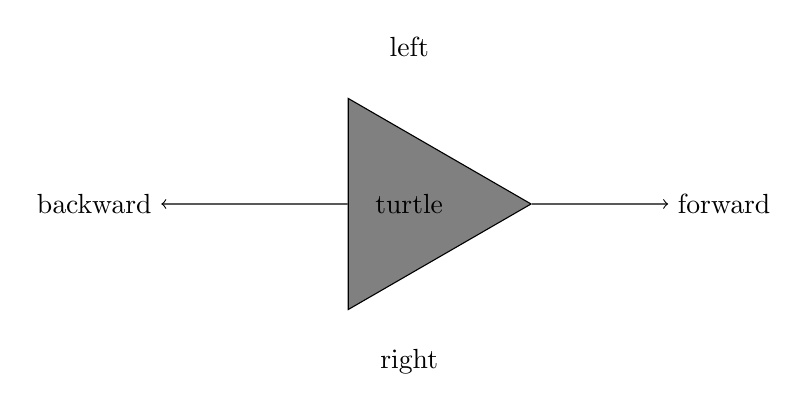
\begin{tikzpicture}

% nodes
\node (bk) at (4, 2) {backward};
\node[turtle] (tt) at (8, 2) {turtle};
\node (fd) at (12, 2) {forward};
\node (lt) at (8, 4) {left};
\node (rt) at (8, 0) {right};

% arrows
\draw[->] (tt) edge (bk);
\draw[->] (tt) edge (fd);

\end{tikzpicture}
\caption{绘图海龟的基本概念}
\end{figure}

许多分形构造或者镶嵌构造可以非常方便的通过一种支持裂解操作的 Logo 语言来实现。我们放宽原始 Logo 语言里的设定,
允许在画布上有多个海龟的存在,并且每个海龟单独维护自己的步长标准。于是,所谓的裂解是指一个操作,
它可以让一个海龟变成按照一定角度排布的多个海龟,同时新生成的海龟有新的步长设定。对于角度的排布,我们规定前进方向右侧转向是正的方向。

\begin{convention}
裂解采用如下的命令形式:
\begin{itemize}
\item 裂解[角度排布;步长设定]
\end{itemize}
\end{convention}

\subsection{四阶无限边形镶嵌}

双曲平面上有许多非常有趣的镶嵌结构,这里我们展示一种称为四阶无限边形镶嵌的构造。

\begin{figure}[ht]
\centering
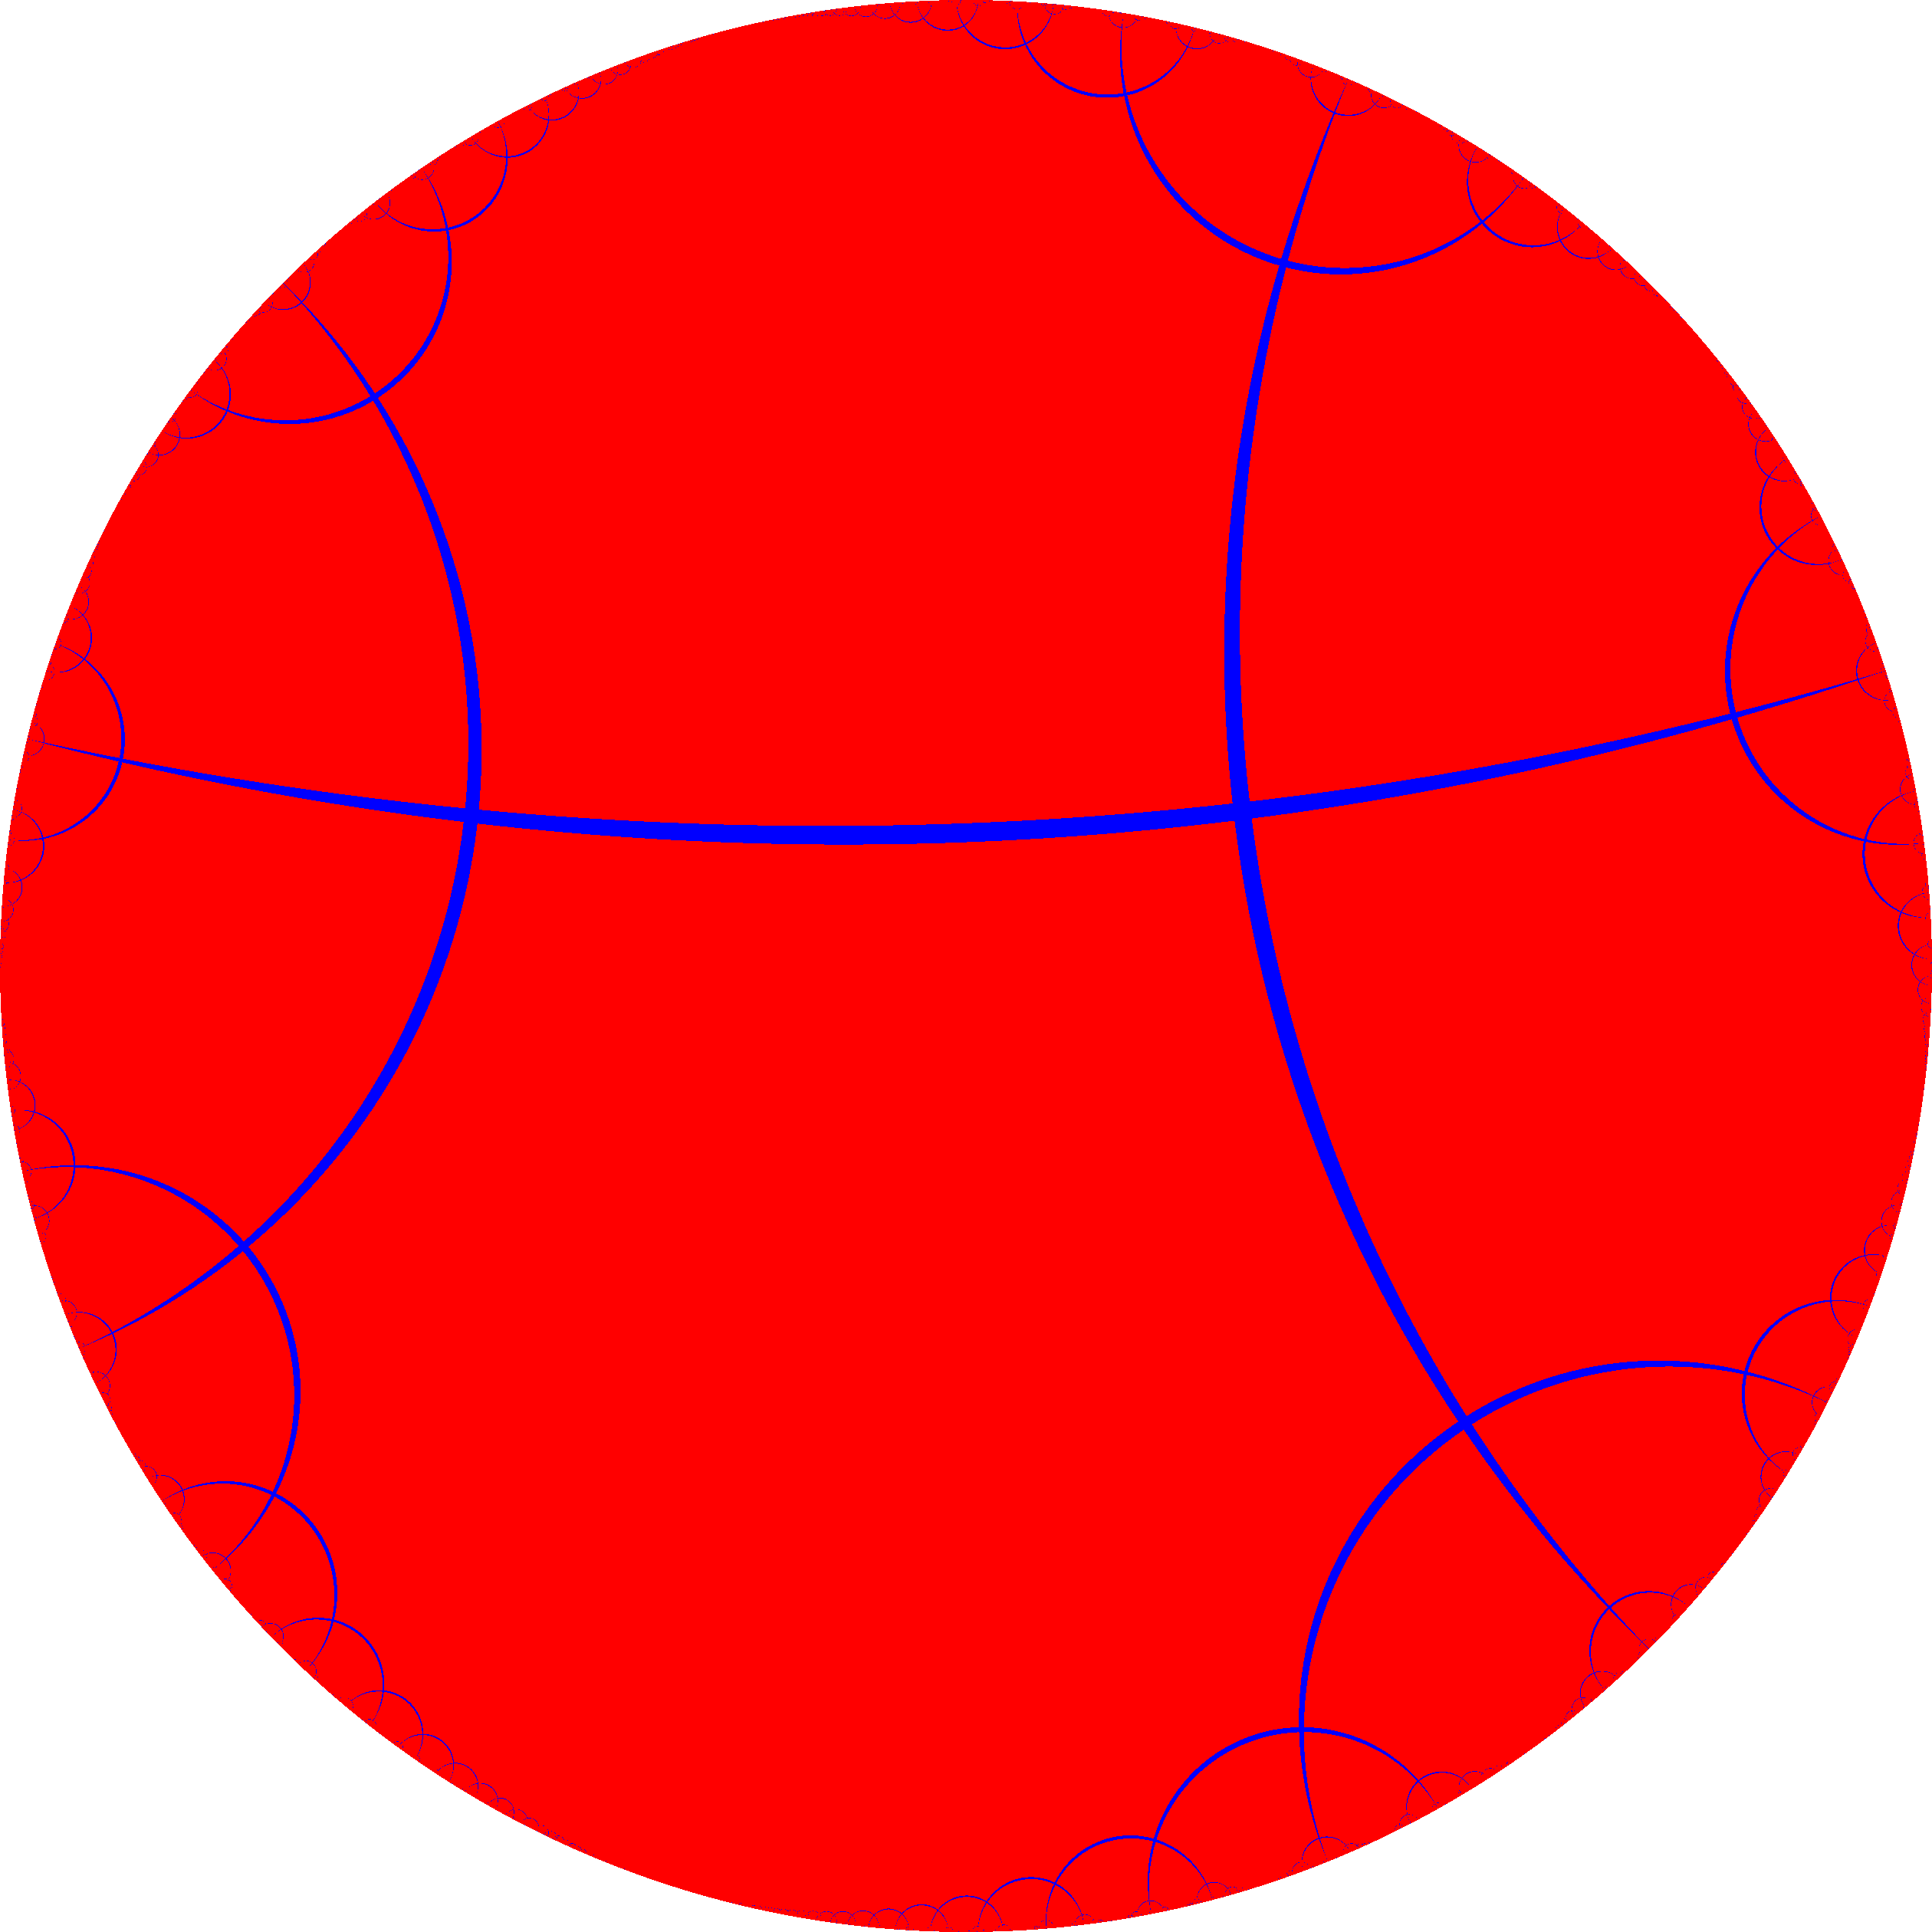
\includegraphics[width=3.5in]{images/H2_tiling_24i-1.png}
\caption{四阶无限边形镶嵌}
\end{figure}

这个镶嵌结构的构造程序如下

\begin{program}
四阶无限边形镶嵌的构造一
\begin{itemize}
\item 裂解[0, +90, +180, +270; 1]
\item 对所有的小海龟,反复无限次的执行下述命令
\begin{itemize}\item 前进一步 \item 裂解[-90, 0, +90; 1] \end{itemize}
\end{itemize}
\end{program}

如果注意到双曲平面是一个齐性空间,并且观察到在上述构造里,有些蓝色测地线之间彼此有交点,但这些交点彼此之间没有任何差别;
每一个交点都是两个测地线交汇出来的,都有四支分叉。利用对称性,我们容易理解:

\begin{proposition}
\label{A}
镶嵌结构上的两条测地线如果彼此之间相交,那么它们就是垂直的;否则这两条测地线就是平行的。
\end{proposition}

\begin{proposition}
\label{B}
对于任意一条镶嵌结构上的测地线,镶嵌结构上的其他测地线可以被归类到与之平行或垂直的两组之中。
\end{proposition}

\subsection{H-树}

H-树是如下图所示的分形构造。四阶无限边形镶嵌按照一定规则剪枝,拓扑上可以得到H-树。

\begin{figure}[ht]
\centering
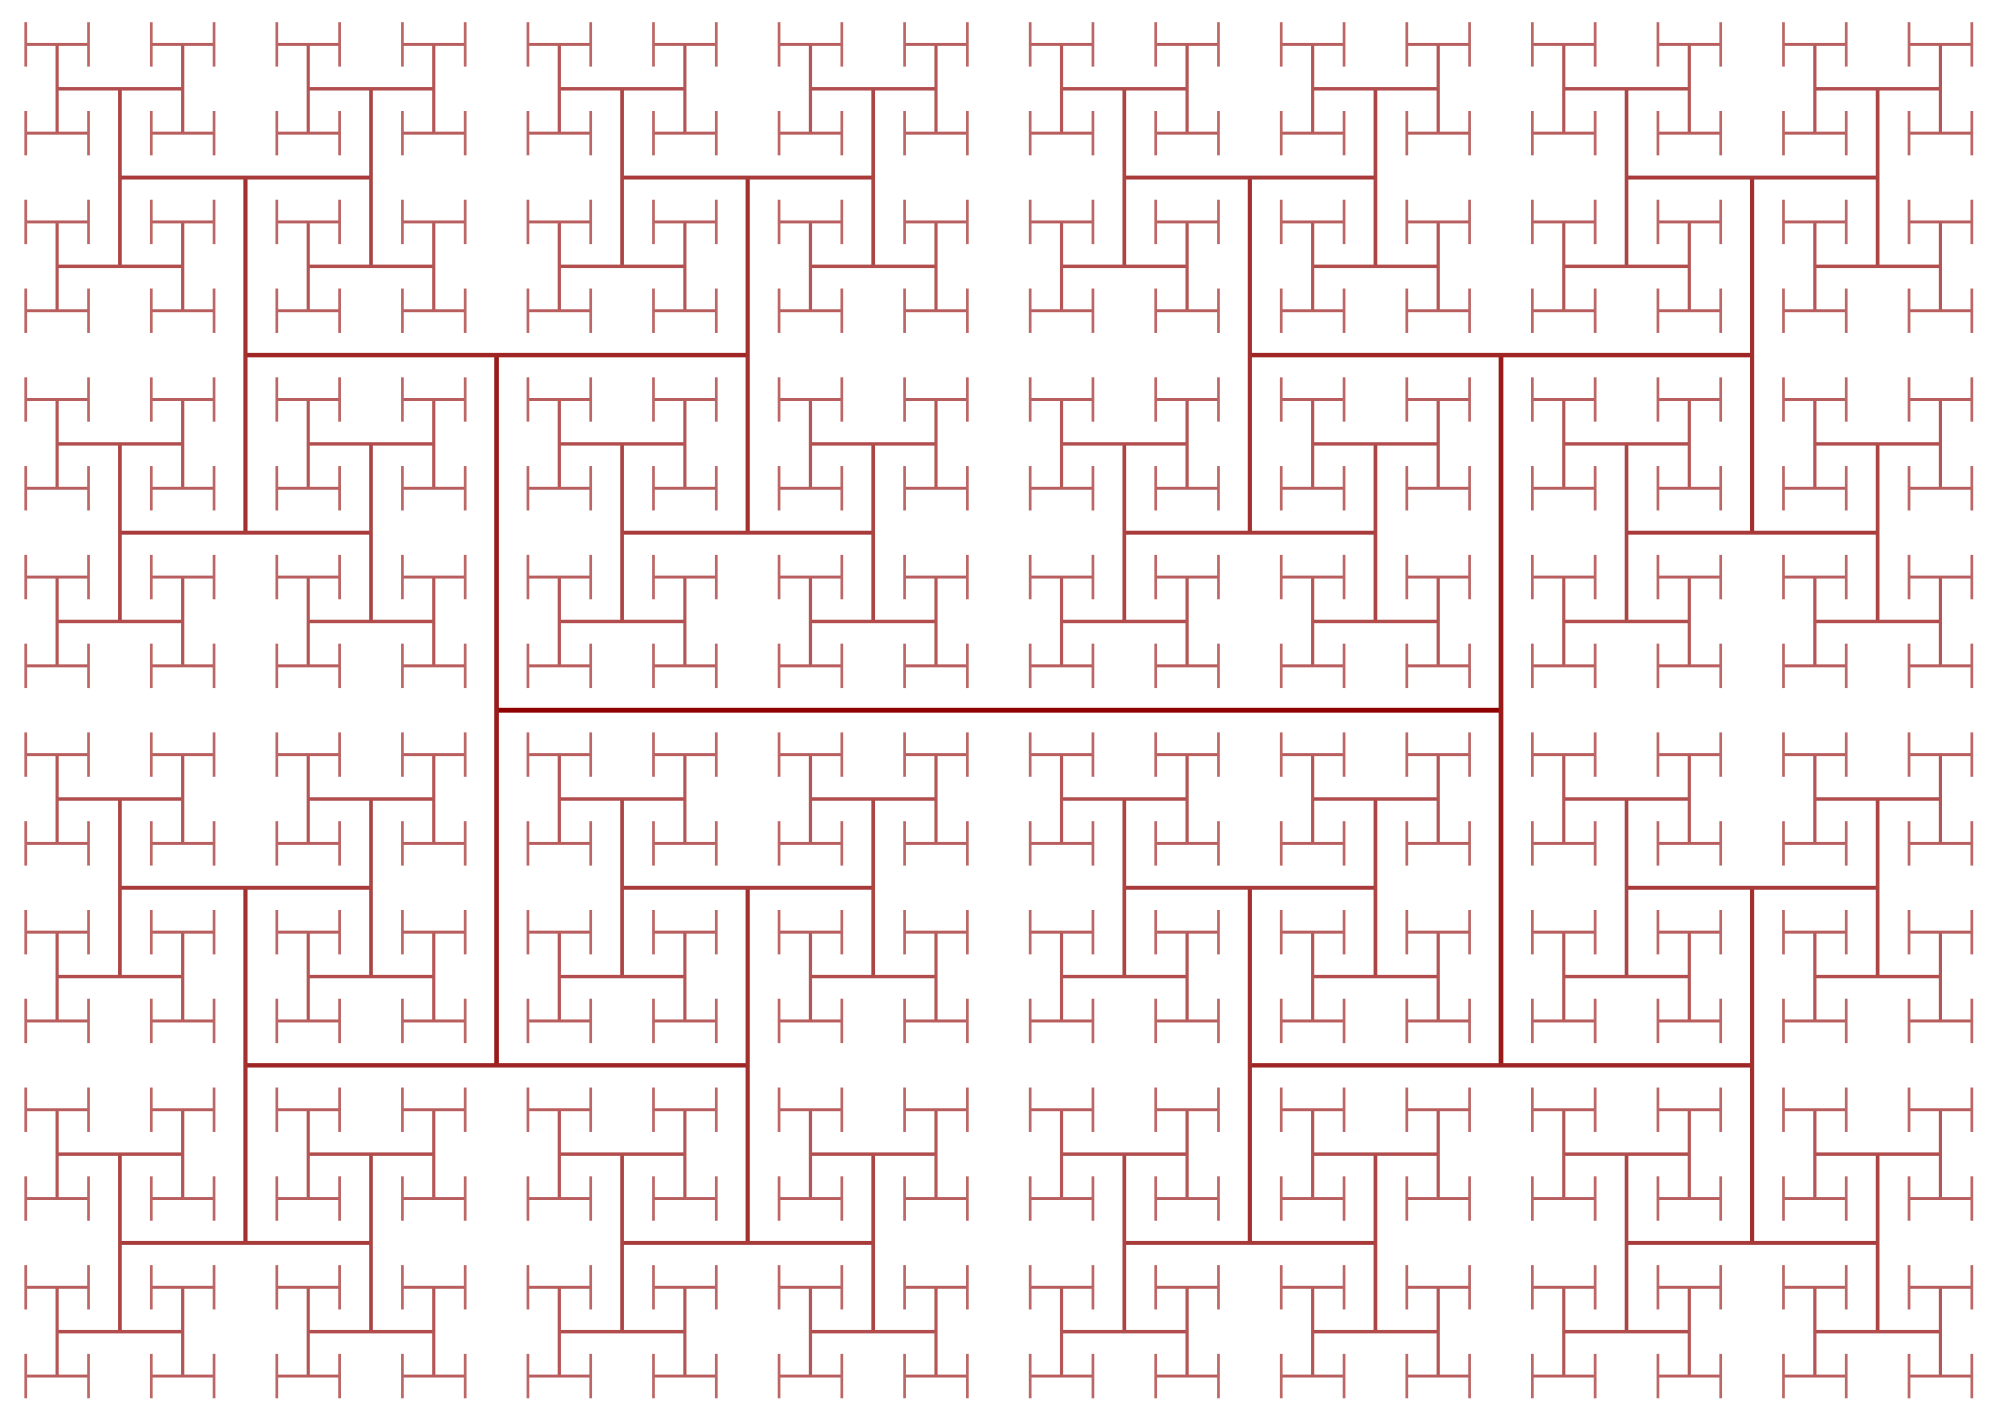
\includegraphics[width=3.5in]{images/2000px-H_tree.png}
\caption{H-树}
\end{figure}

H-树的具体构造程序如下

\begin{program}
H-树的构造
\begin{itemize}
\item 对所有的小海龟,反复无限次的执行下述命令
\begin{itemize}\item 前进一步 \item 裂解[-90, +90; $\sqrt{2} / 2$] \end{itemize}
\end{itemize}
\end{program}

\newpage

\section{不同的赋值方案}

\subsection{第一种赋值方案}

下面我们给四阶无限边形镶嵌的边着色。着色的基本原则是前进方向的右侧是 b 或者 w,前进方向的左侧是 d 或者 m;同时,b 和 d 作为加性组,
m 和 w 作为乘性组,它们彼此交替出现。上述过程可以被下面的程序刻画。

\begin{figure}[ht]
\centering
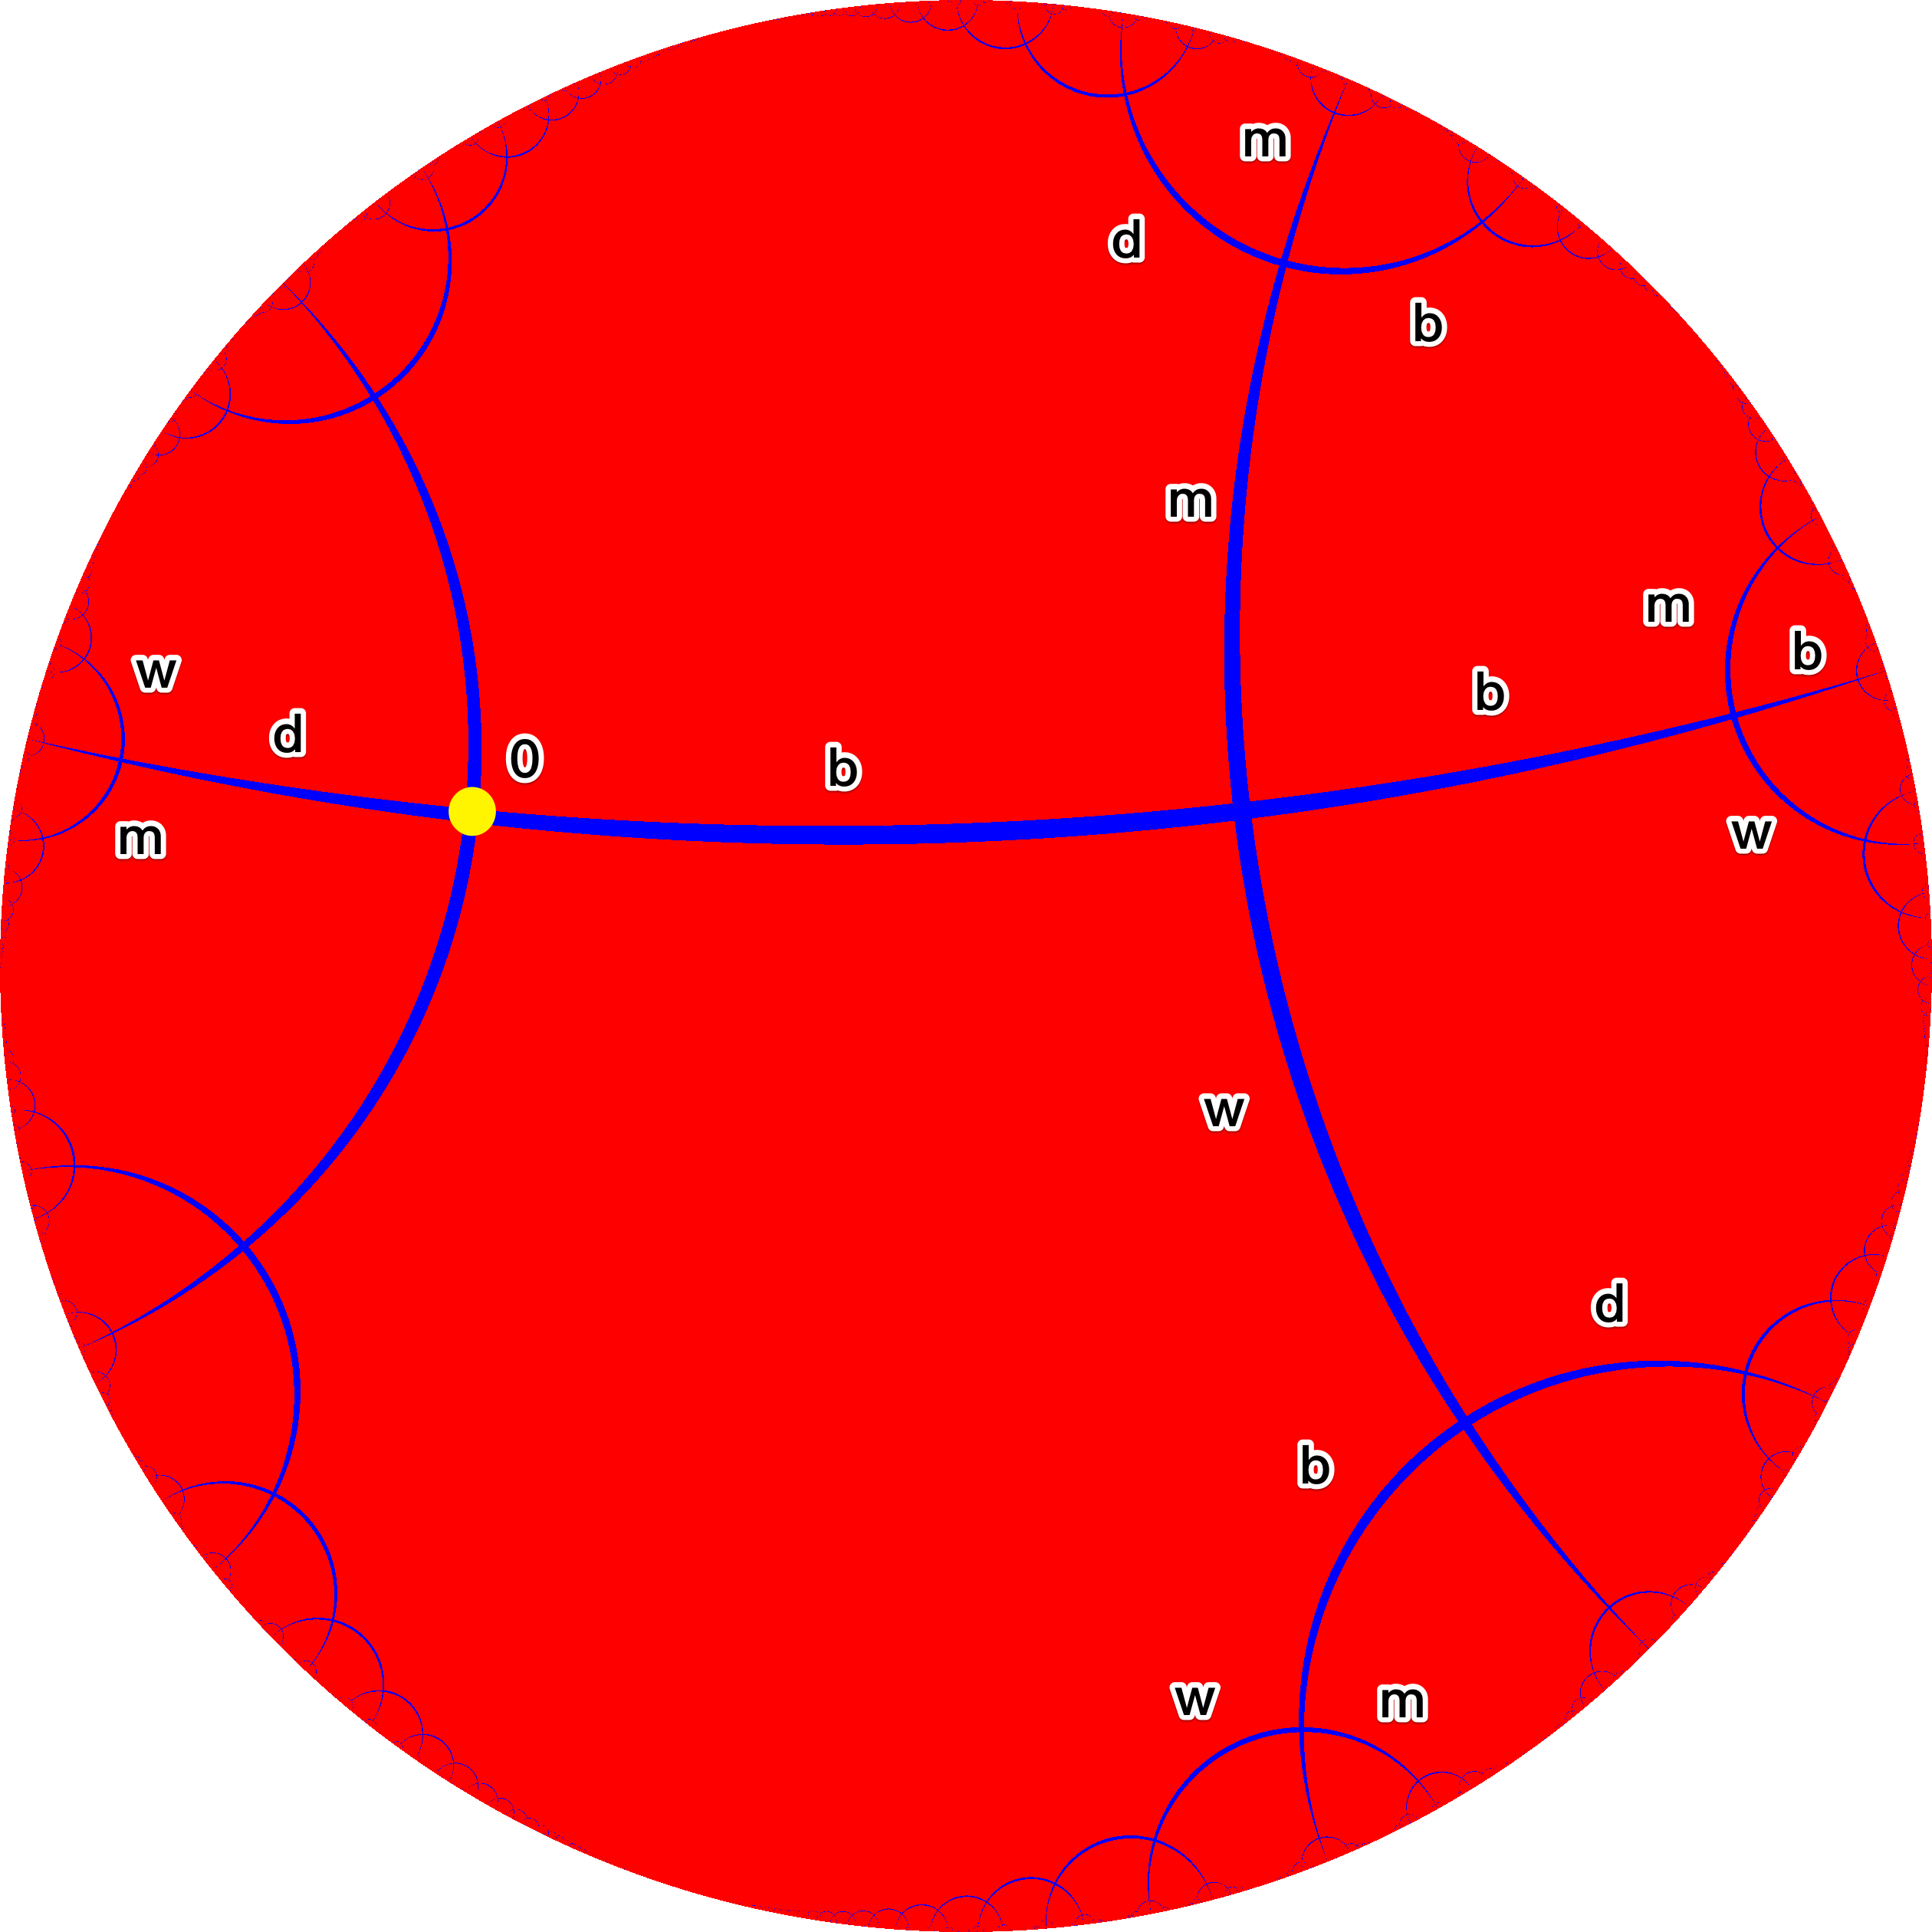
\includegraphics[width=3.5in]{images/H2_tiling_with_color_1.png}
\caption{在边上着色}
\end{figure}

\begin{program}
四阶无限边形镶嵌的着色方案一
\begin{itemize}
\item 裂解[0, +90, +180, +270; 1],朝向 0 度的小海龟背着符号 b,朝向 180 度的小海龟背着符号 d,朝向 90 度的是 m,朝向 270 度的是 w。
\item 对所有的小海龟,反复无限次的执行下述命令
\begin{itemize}
  \item 前进一步
  \item 裂解[-90, 0, +90; 1],朝向 0 度的小海龟背着的符号不变,其余小海龟背着的符号做出变化如下
    \begin{itemize}
      \item 如果裂解前海龟背着 b 或者 d,则朝向 -90 度的小海龟背着 m,朝向 90 度的小海龟背着 w
      \item 如果裂解前海龟背着 m 或者 w,则朝向 -90 度的小海龟背着 d,朝向 90 度的小海龟背着 b
    \end{itemize}
  \end{itemize}
\end{itemize}
\end{program}

上述程序执行的起点是给定的零点 O。对镶嵌上的任何一点 A,从 O 到 A 只有唯一的一条路径,我们把该路径上边的着色拼接起来,再加上起点的 0,
就得到一个 文法\ref{g1} 描述的表达式,这个表达式的值给点 A 一个赋值。

\begin{figure}[ht]
\centering
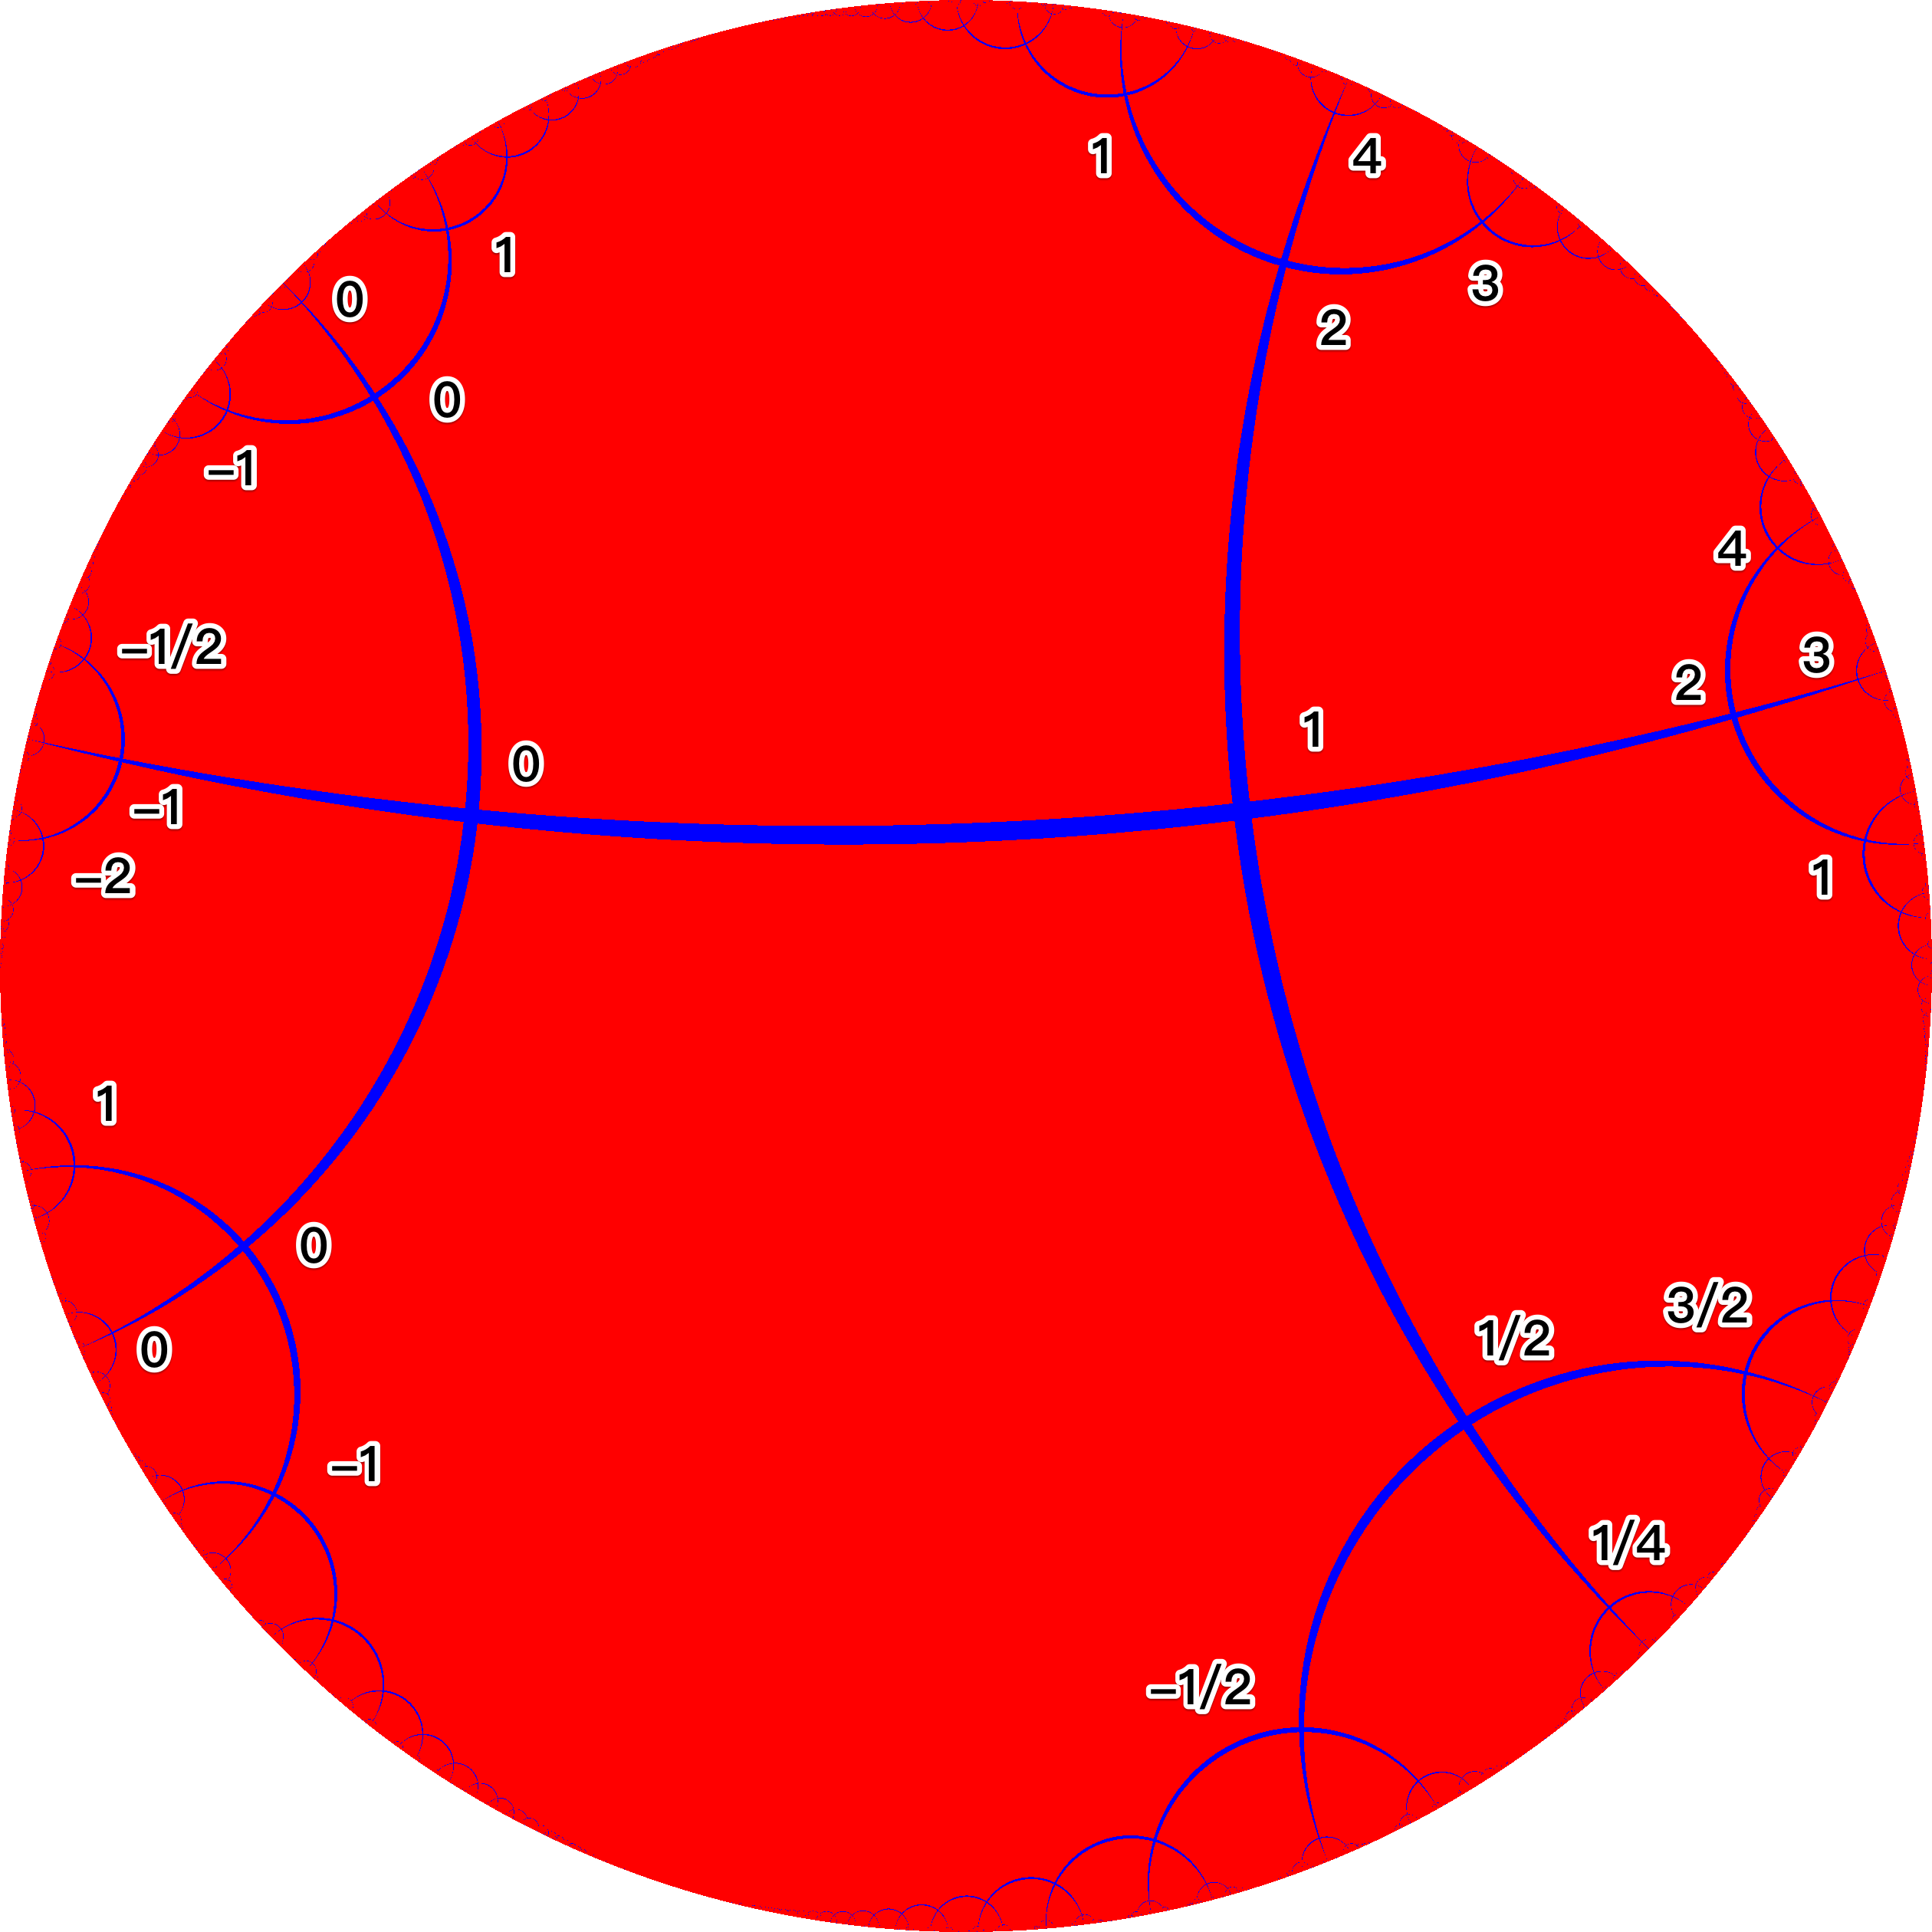
\includegraphics[width=3.5in]{images/H2_tiling_with_assign_1.png}
\caption{镶嵌上的第一种赋值}
\end{figure}

需要指出的是,由于 引理\ref{l1} 的存在,上述赋值是恰当的。(恰当性还需要进一步论述,特别是如果我们考虑了赋值后的镶嵌图案的内在对称性的时候)

\subsection{第二种赋值方案}

在第 1.1 节,我们曾经考虑了一个自然数的最简表达。在本节,我们引入特殊的零点,让符号性质的最简表达,有一个自然的几何表示—最短路径。

\subsubsection{一个特殊零点的引入}

我们还有四阶无限边形镶嵌的另外一种构造程序,这个构造引入了一个特殊的零点。

\begin{program}
四阶无限边形镶嵌的构造二
\begin{itemize}
\item 裂解[0, +180; 1]
\item 前进半步
\item 对所有的小海龟,反复无限次的执行下述命令
\begin{itemize}
  \item 前进一步
  \item 裂解[-90, 0, +90; 1]
\end{itemize}
\end{itemize}
\end{program}

上述程序里小海龟的起点就是我们特殊的零点。

\begin{figure}[ht]
\centering
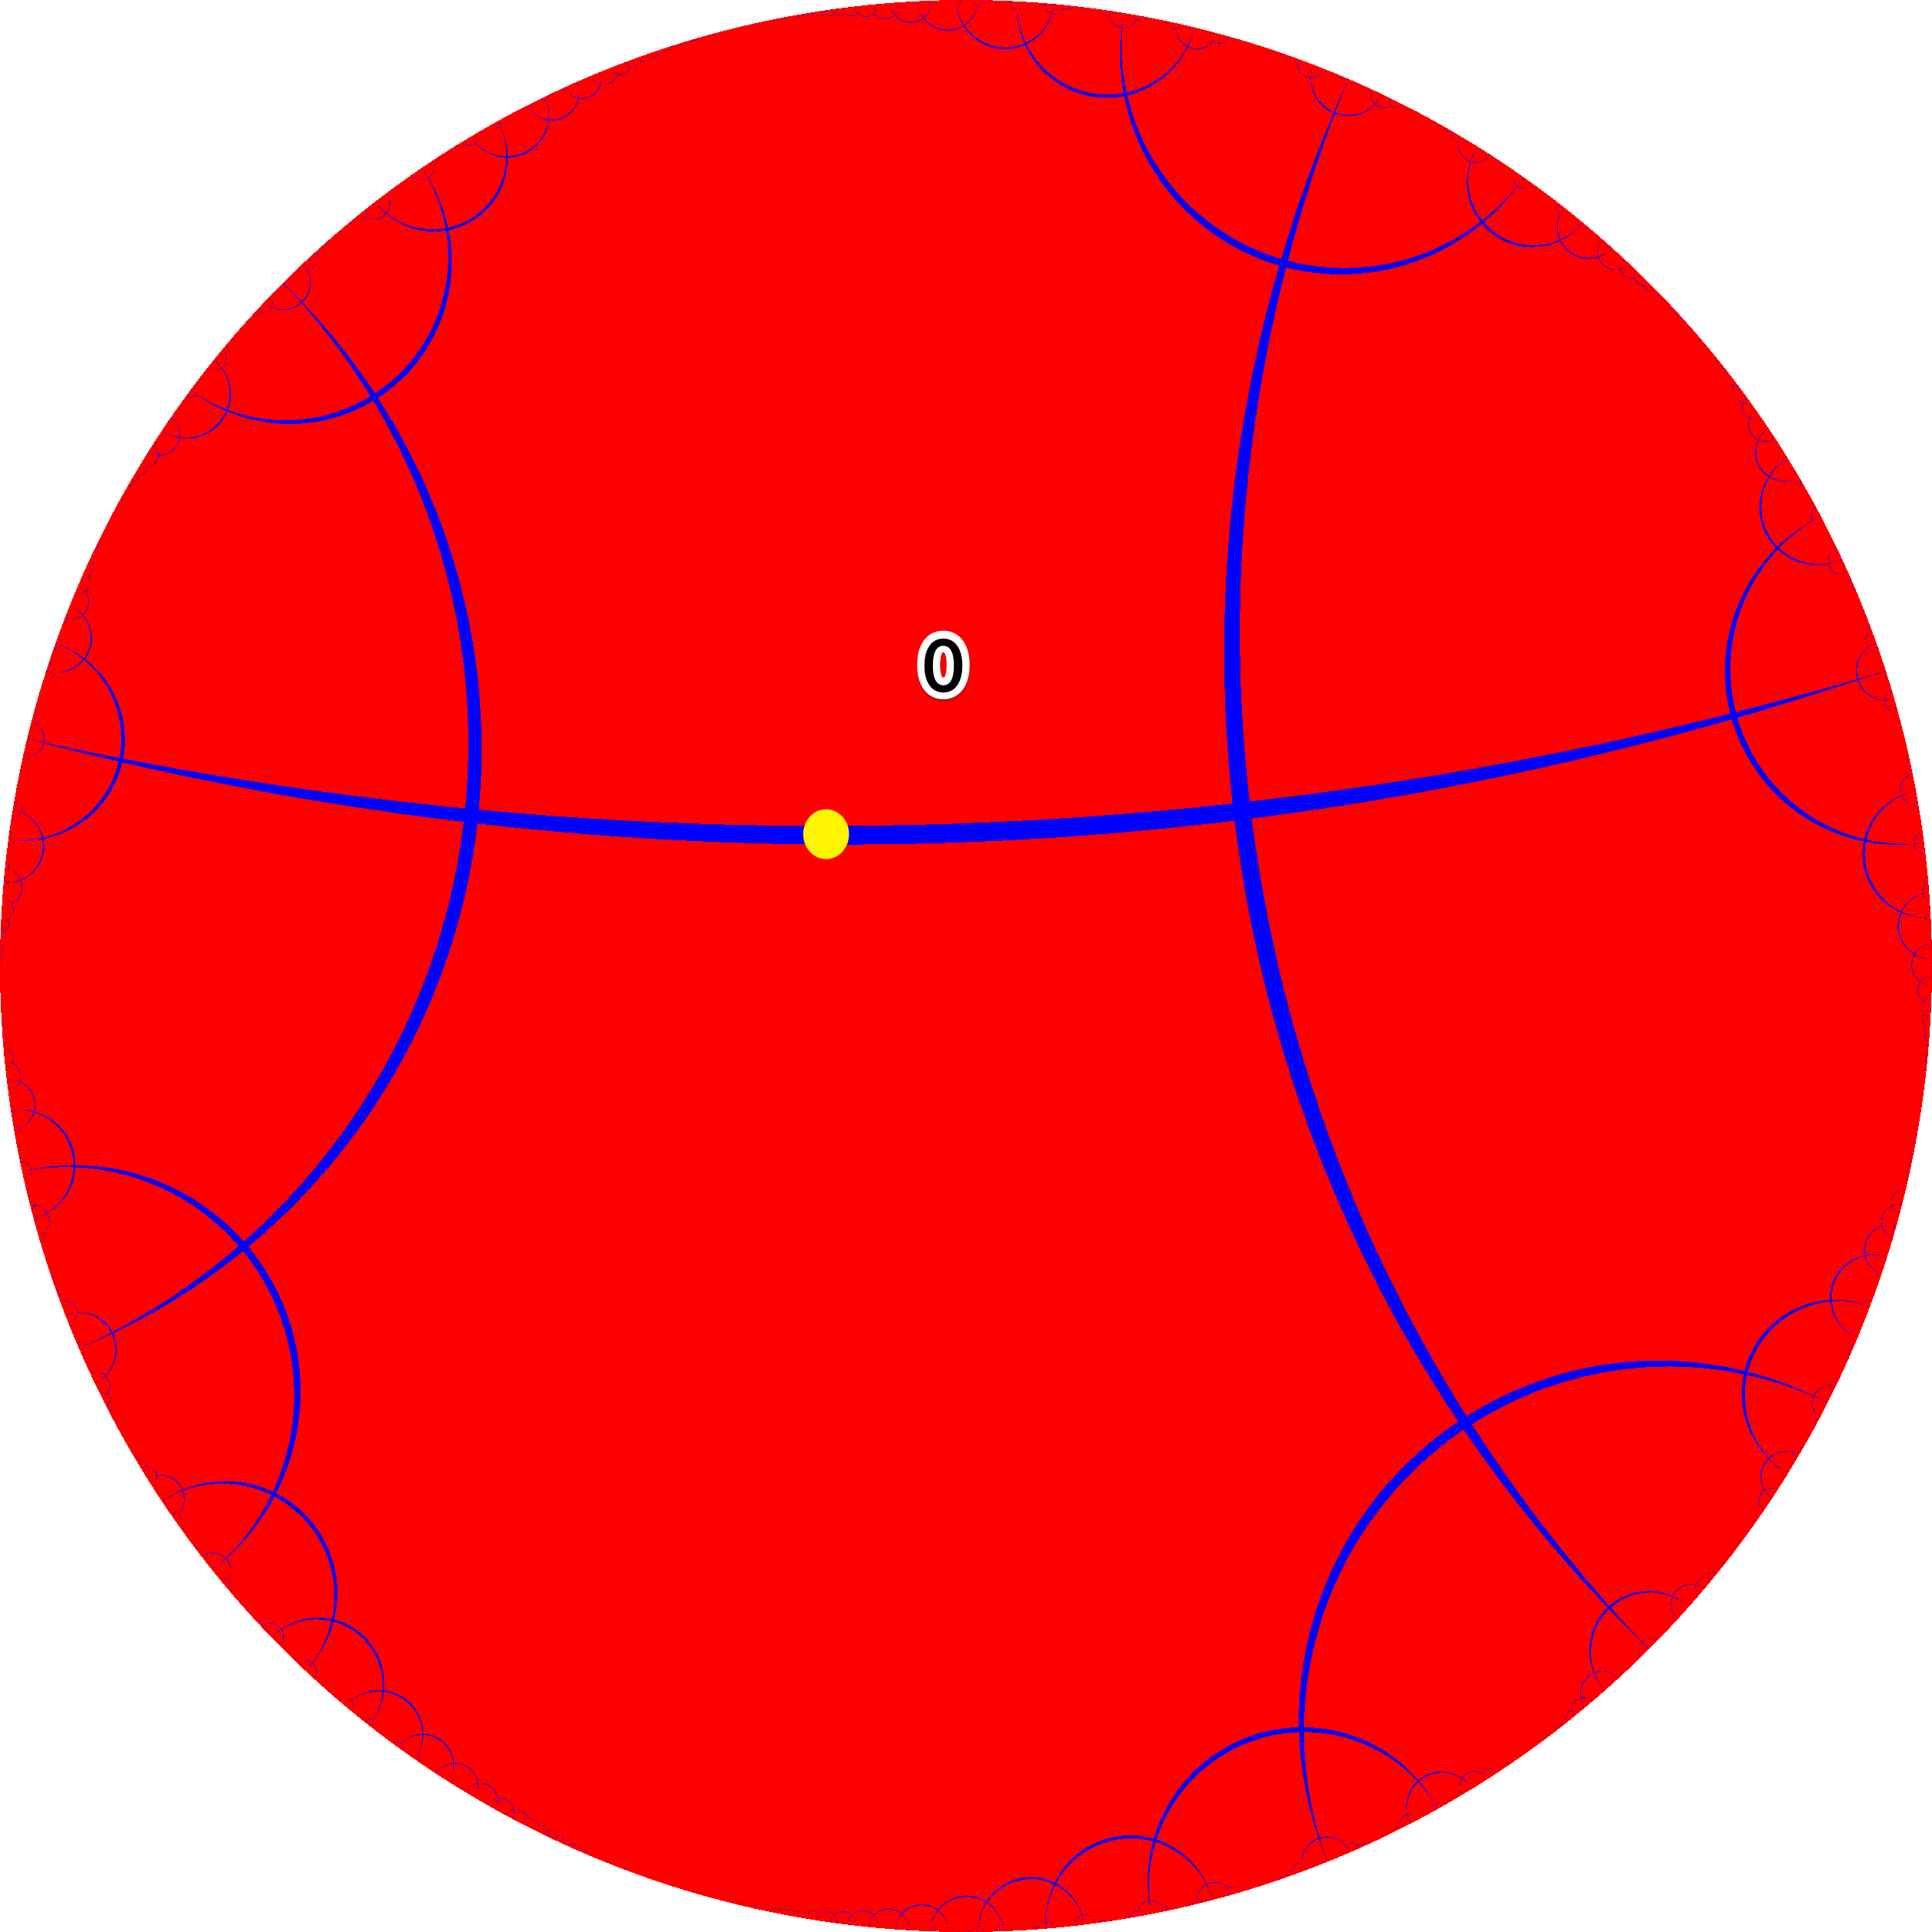
\includegraphics[width=3.5in]{images/H2_tiling_with_zero_2.png}
\caption{一个特殊零点的引入}
\end{figure}

\subsubsection{着色方案一的小修正}

基本沿用着色方案一,只作非常小的修正,我们给出如下的程序。

\begin{figure}[ht]
\centering
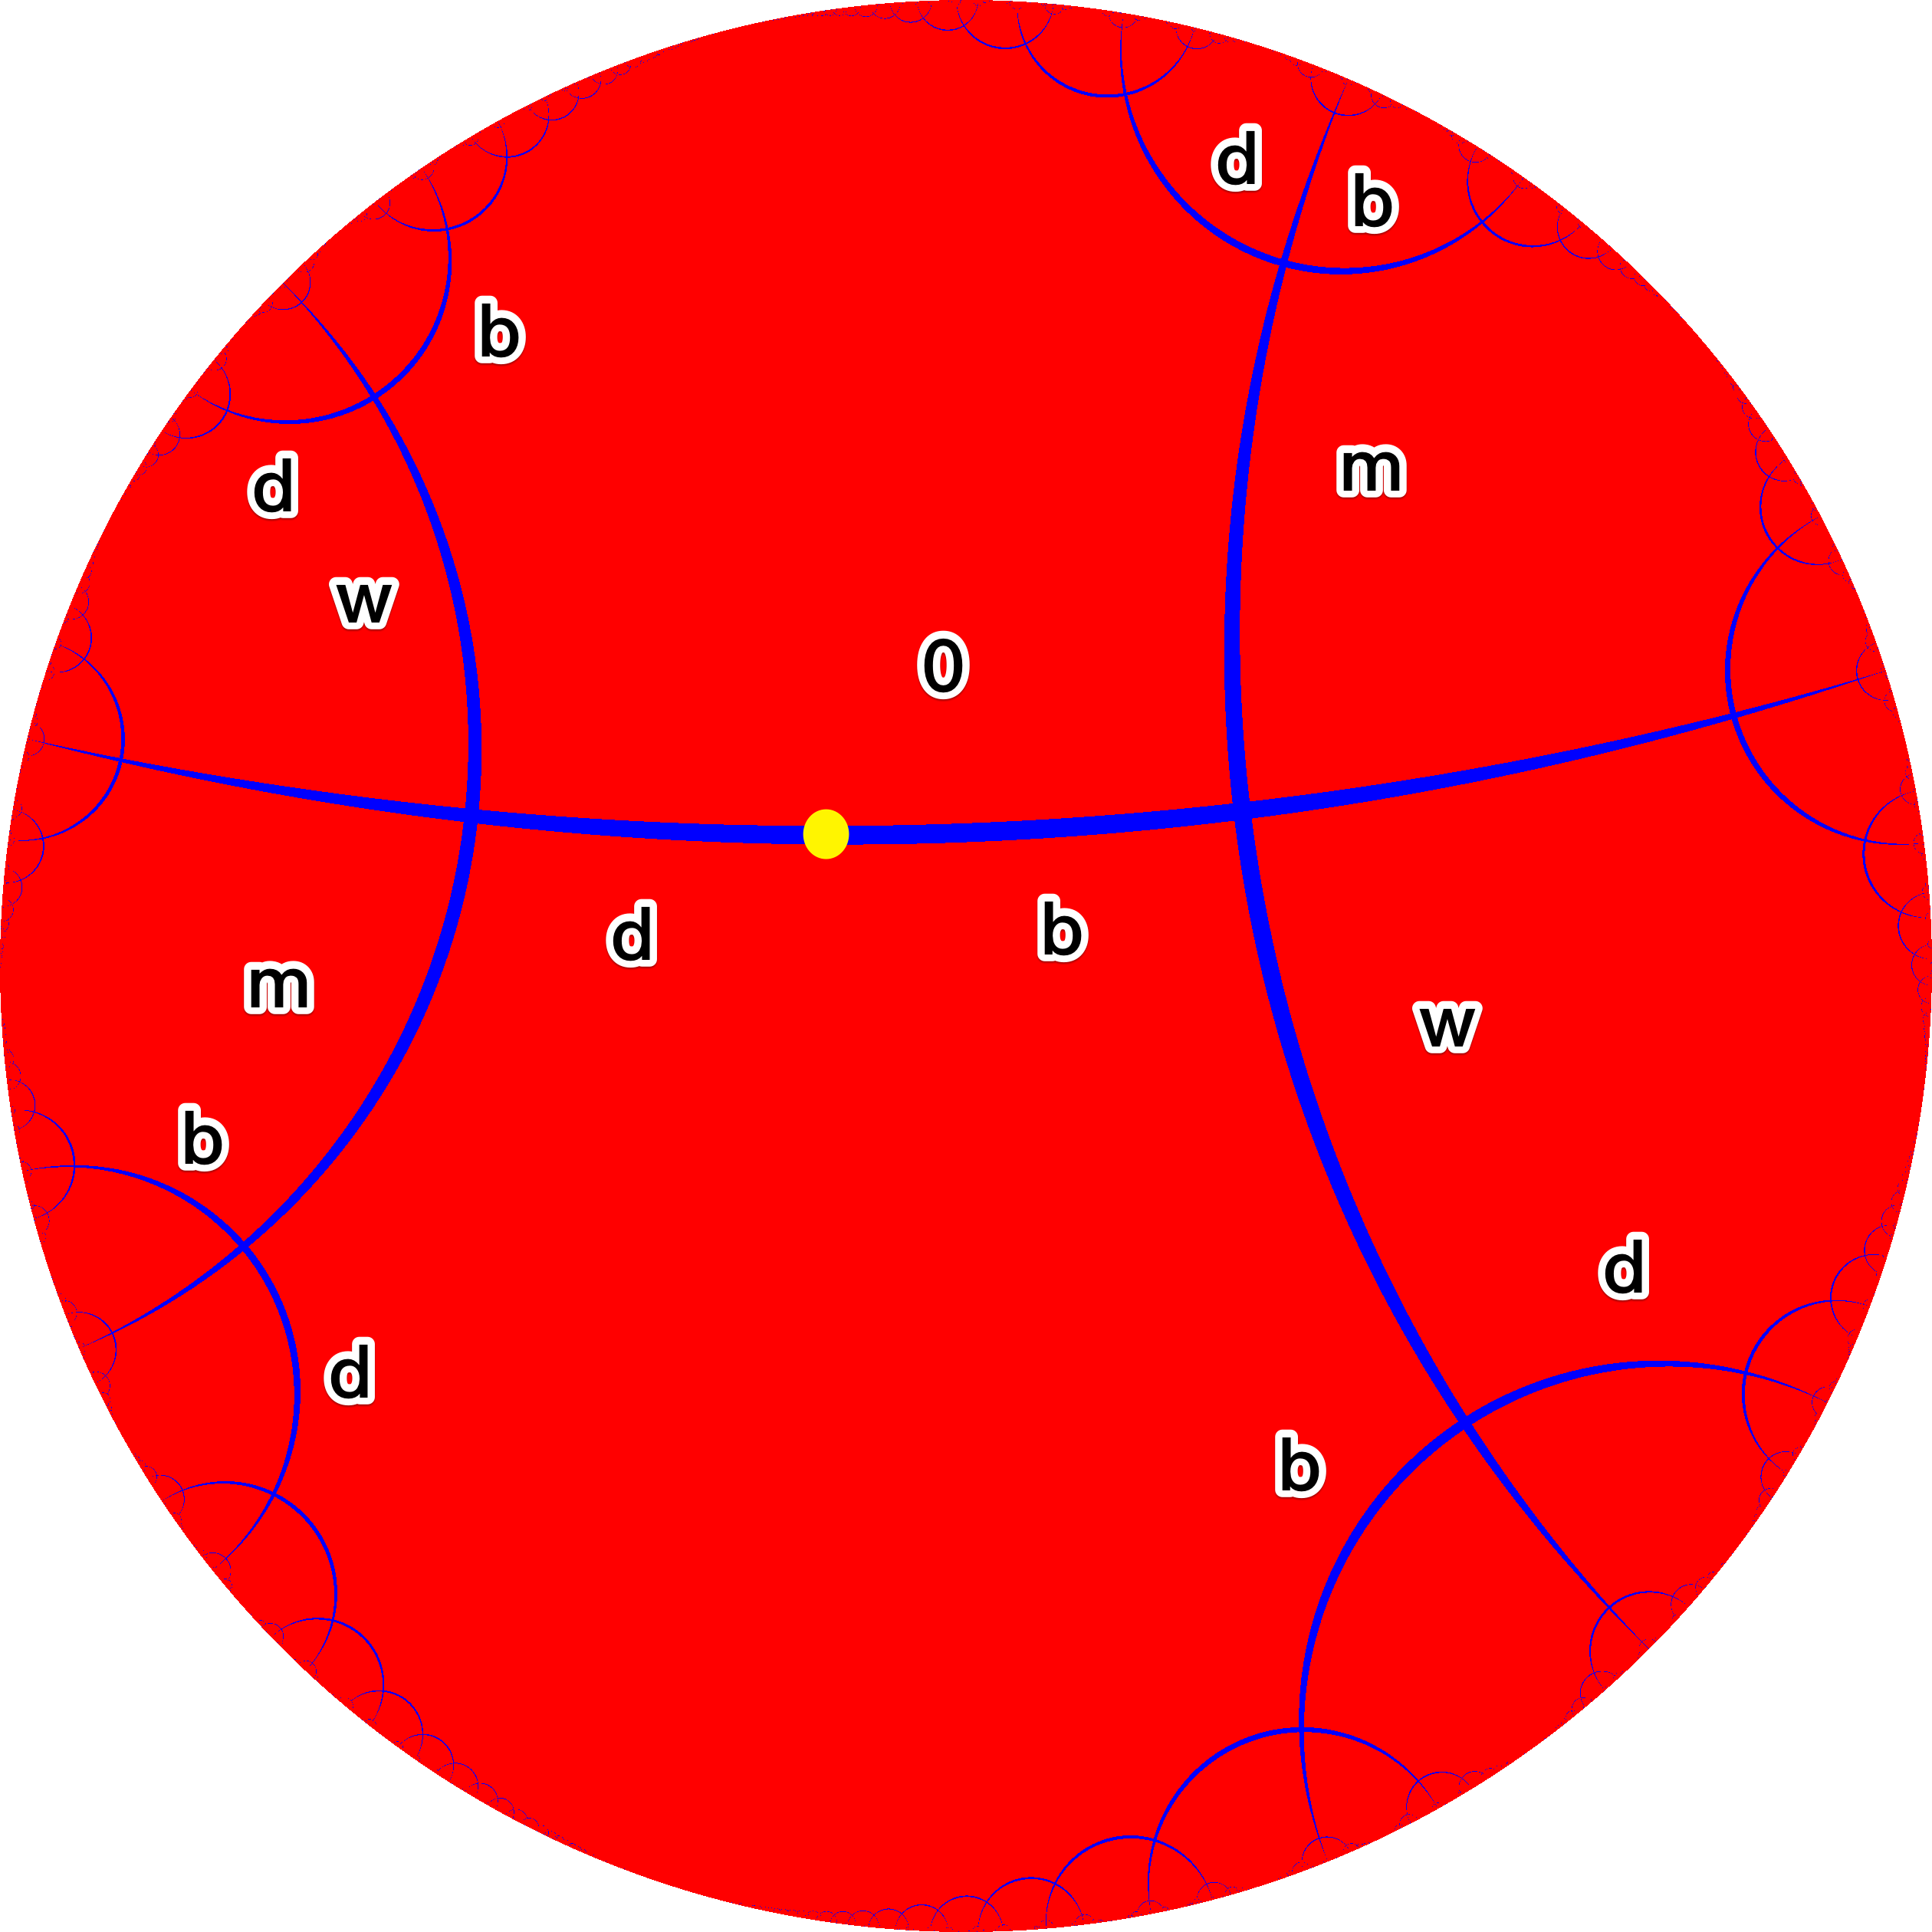
\includegraphics[width=3.5in]{images/H2_tiling_with_color_2.png}
\caption{着色方案一的小修正}
\end{figure}

\begin{program}
着色方案一的小修正
\begin{itemize}
\item 裂解[0, +180; 1],朝向 0 度的小海龟背着符号 b,朝向 180 度的小海龟背着符号 d
\item 前进半步
\item 对所有的小海龟,反复无限次的执行下述命令
\begin{itemize}
  \item 前进一步
  \item 裂解[-90, 0, +90; 1],朝向 0 度的小海龟背着的符号不变,其余小海龟背着的符号做出变化如下
    \begin{itemize}
      \item 如果裂解前海龟背着 b 或者 d,则朝向 -90 度的小海龟背着 m,朝向 90 度的小海龟背着 w
      \item 如果裂解前海龟背着 m 或者 w,则朝向 -90 度的小海龟背着 d,朝向 90 度的小海龟背着 b
    \end{itemize}
  \end{itemize}
\end{itemize}
\end{program}

稍微思考一下,就会发现这种方案的不足:零点会出现无限次,但它们彼此并不等同。
这就要求我们,对所有的零点都必须特殊处理,当走到 1 或者 -1 时,必须要前进或者后退半步,来得到新的零点。

\subsubsection{更优的方案}

我们增强小海龟的装备,除了能背负 b、d、m、w 四种颜色;它还背负了一个计算器—
当小海龟从零点走到当前点,它的计算器能够计算路径的估值是多少。

\begin{program}
更优的着色方案
\begin{itemize}
    \item 反复无限次的执行下述命令
    \begin{itemize}
        \item 对所有的在零点的小海龟:
        \begin{itemize}
            \item 裂解[0, +180; 1],朝向 0 度的小海龟背着符号 b,朝向 180 度的小海龟背着符号 d
            \item 如果前方的边没有被着色,则前进半步,否则保持不动
        \end{itemize}
        \item 对所有的不在零点的小海龟
        \begin{itemize}
            \item 当前的位置上路径的估值不为 1 或者 -1
            \begin{itemize}
                \item 前进一步
                \item 裂解[-90, 0, +90; 1],朝向 0 度的小海龟背着的符号不变,其余小海龟背着的符号做出变化如下:
                    如果裂解前海龟背着 b 或者 d,则朝向 -90 度的小海龟背着 m,朝向 90 度的小海龟背着 w;
                    如果裂解前海龟背着 m 或者 w,则朝向 -90 度的小海龟背着 d,朝向 90 度的小海龟背着 b。
            \end{itemize}
            \item 当前的位置上路径的估值为 1 且海龟背着 d,则前进半步,停在一个新的零点,小海龟的指向翻转
            \item 当前的位置上路径的估值为 -1 且海龟背着 b,则前进半步,停在一个新的零点,小海龟的指向不变
        \end{itemize}
    \end{itemize}
\end{itemize}
\end{program}

更优的着色方案会给出第二种赋值方案。

\begin{figure}[ht]
\centering
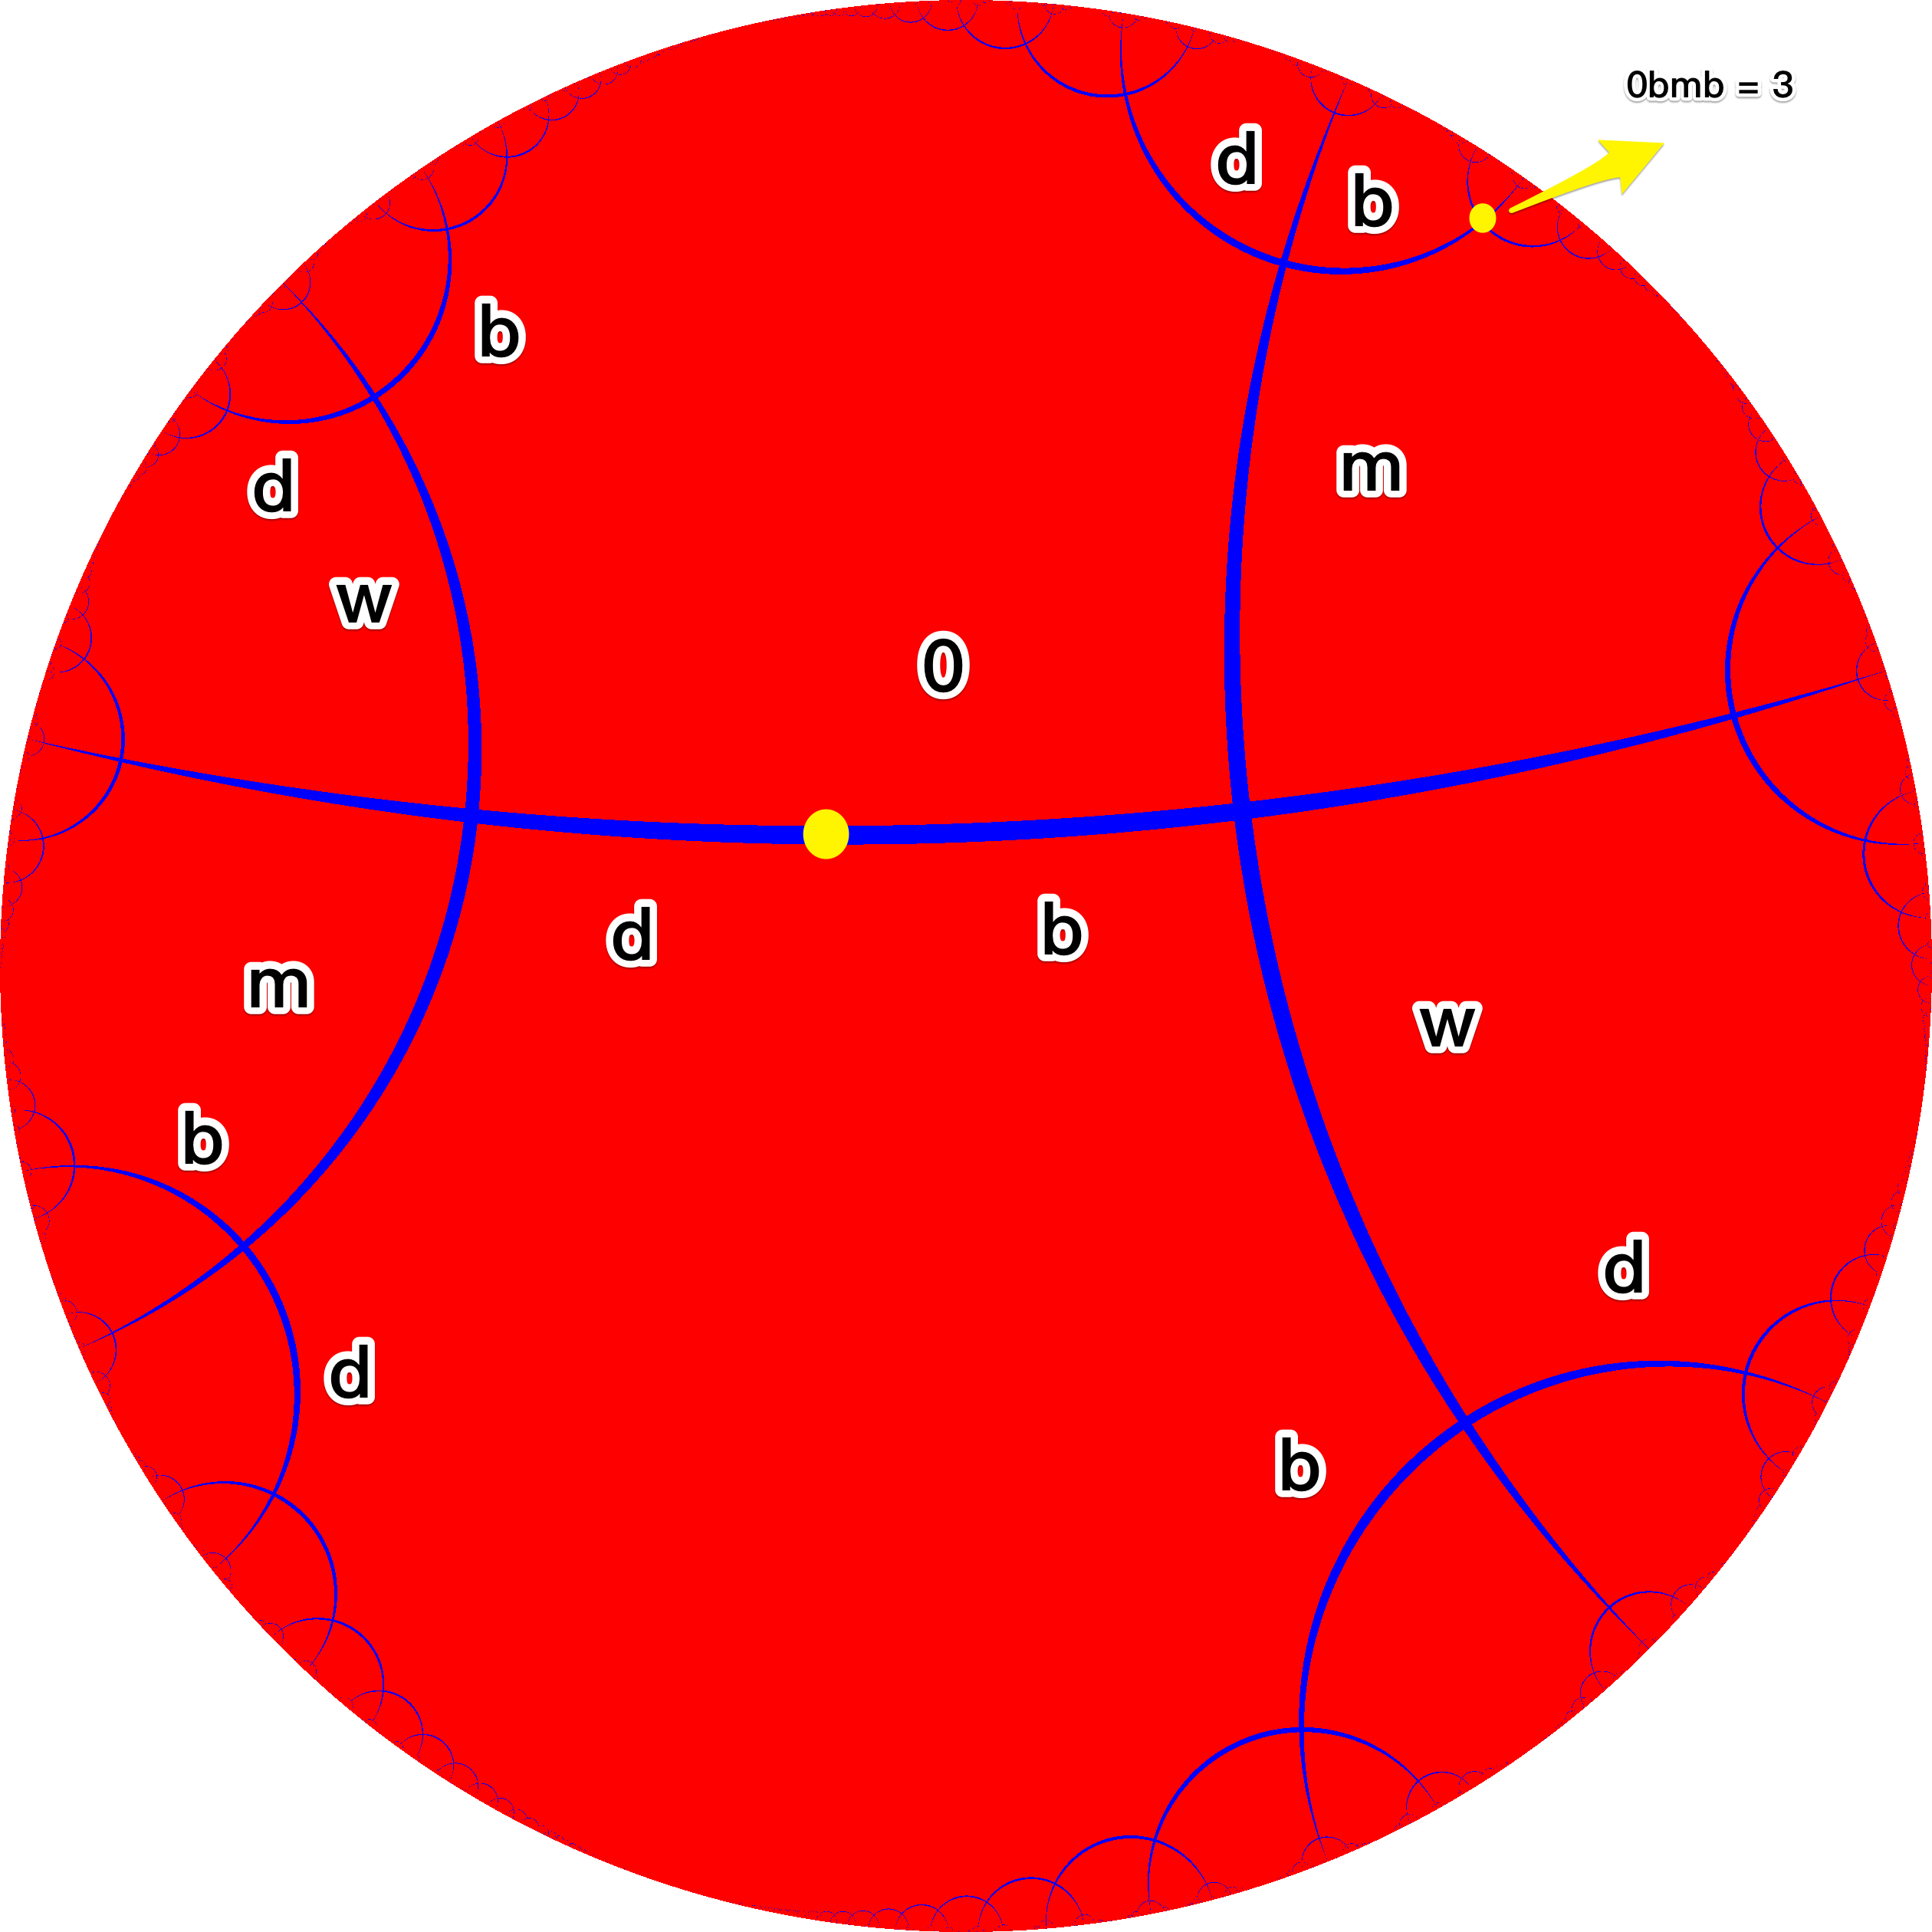
\includegraphics[width=3.5in]{images/H2_tiling_with_assign_2.png}
\caption{第二种赋值方案}
\end{figure}

\section{赋值上的特殊子树}

单调支集

H-支集

给定一个零点,给定一个数字 n,考察所有的 n 对应的点到该零点的路径。需要考察路径中首次出现的 n。
给定一个数字 n 的点,考察所有的零点到该点的路径。需要考察路径中首次出现的零点。

\section{赋值上的模式}

乘法的基

\section{关于赋值的对称群}

\subsubsection{赋值的对称群的存在}

我们知道四阶无限边形镶嵌有一个无限多元素的对称群,如果赋值存在一个对称群,那么一定是它的子群。我们首先来论证这个子群是非平凡的,包含了无限多的元素。
赋值上的所有零点,确定了它的构造。

\section{关于最短表示}

在第二种赋值方案里,对一个数字,我们考察零点到它的最短路径,这个最短路径称为该数字的最短表示。
这个最短表示和该数字的二进制表示之间有对应的关系。

\section{三个研究的方向}

1.研究四阶无限边形镶嵌上赋值的对称群

2.研究数字的新表示,加法和乘法如何在新表示上计算,它们的复杂度是多少?

3.确认是否和 Surreal 数之间有一定的关联?

\newpage

\section{共形映射的想法}

\subsection{嵌入$n$}

\begin{figure}[ht]
\centering
\begin{tikzpicture}
    \draw (0, 0) node[inner sep=0] {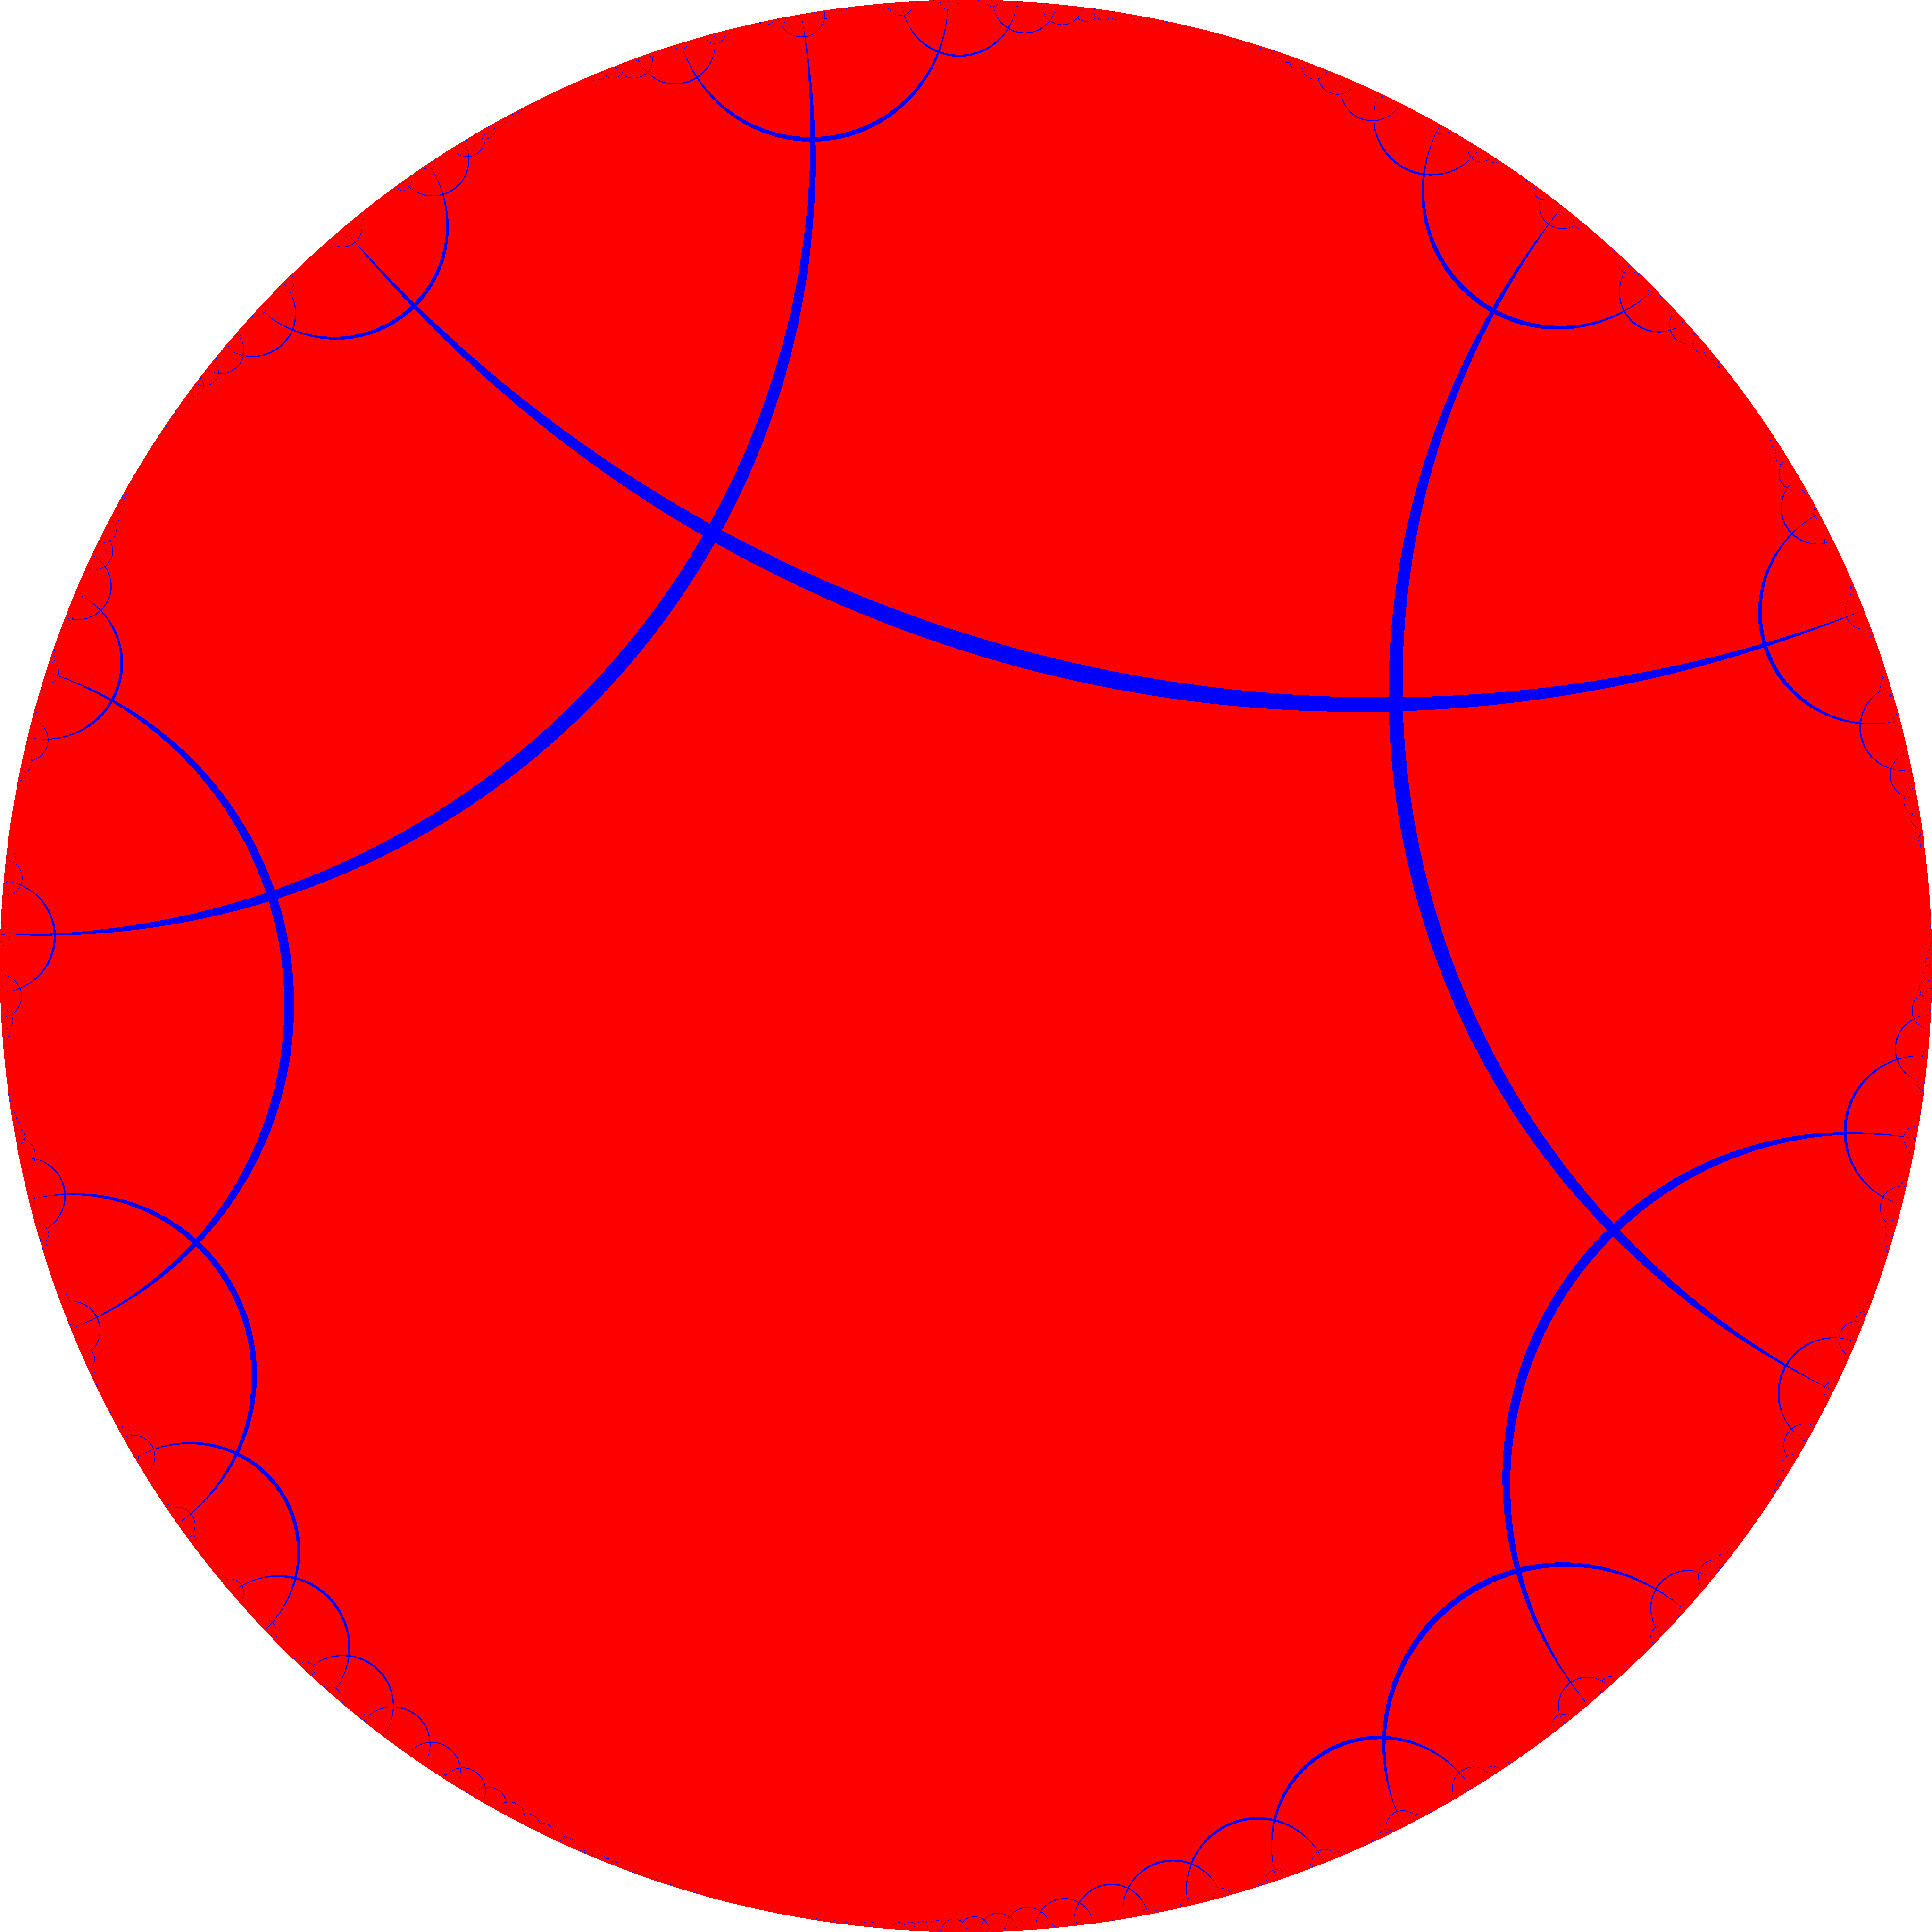
\includegraphics[width=6in]{images/t4096.png}};
    \draw (+1.89, +7.89) node[inner sep=1pt] (p_0) {$-\infty$};
    \draw (+0.90, +5.50) node[inner sep=1pt] (p_0) {0};
    \draw (+0.00, +1.85) node[inner sep=1pt] (p_1) {1};
    \draw (-1.89, -7.89) node[inner sep=1pt] (p_1) {$+\infty$};

    \draw [Black, dotted, thick]
          (-1.89, -7.39) node[inner sep=1pt] (p_pinf) {}
       -- (+1.89, +7.39) node[inner sep=1pt] (p_ninf) {};

    % line 0 %
    \draw [green, dotted, thick]
          (-3.29, 6.84) arc  (240:271.7:18.00);

   % line 1 %
    \draw [green, dotted, thick]
          (-6.43, 4.05) arc  (240:271.7:26.50);

   % line 2 %
    \draw [green, dotted, thick]
          (-7.53, -0.95) arc  (240:271.9:25.70);

\end{tikzpicture}
\caption{嵌入$n$}
\end{figure}

\subsection{嵌入$2^{-n}$}

\begin{figure}[ht]
\centering
\begin{tikzpicture}
    \draw (0, 0) node[inner sep=0] {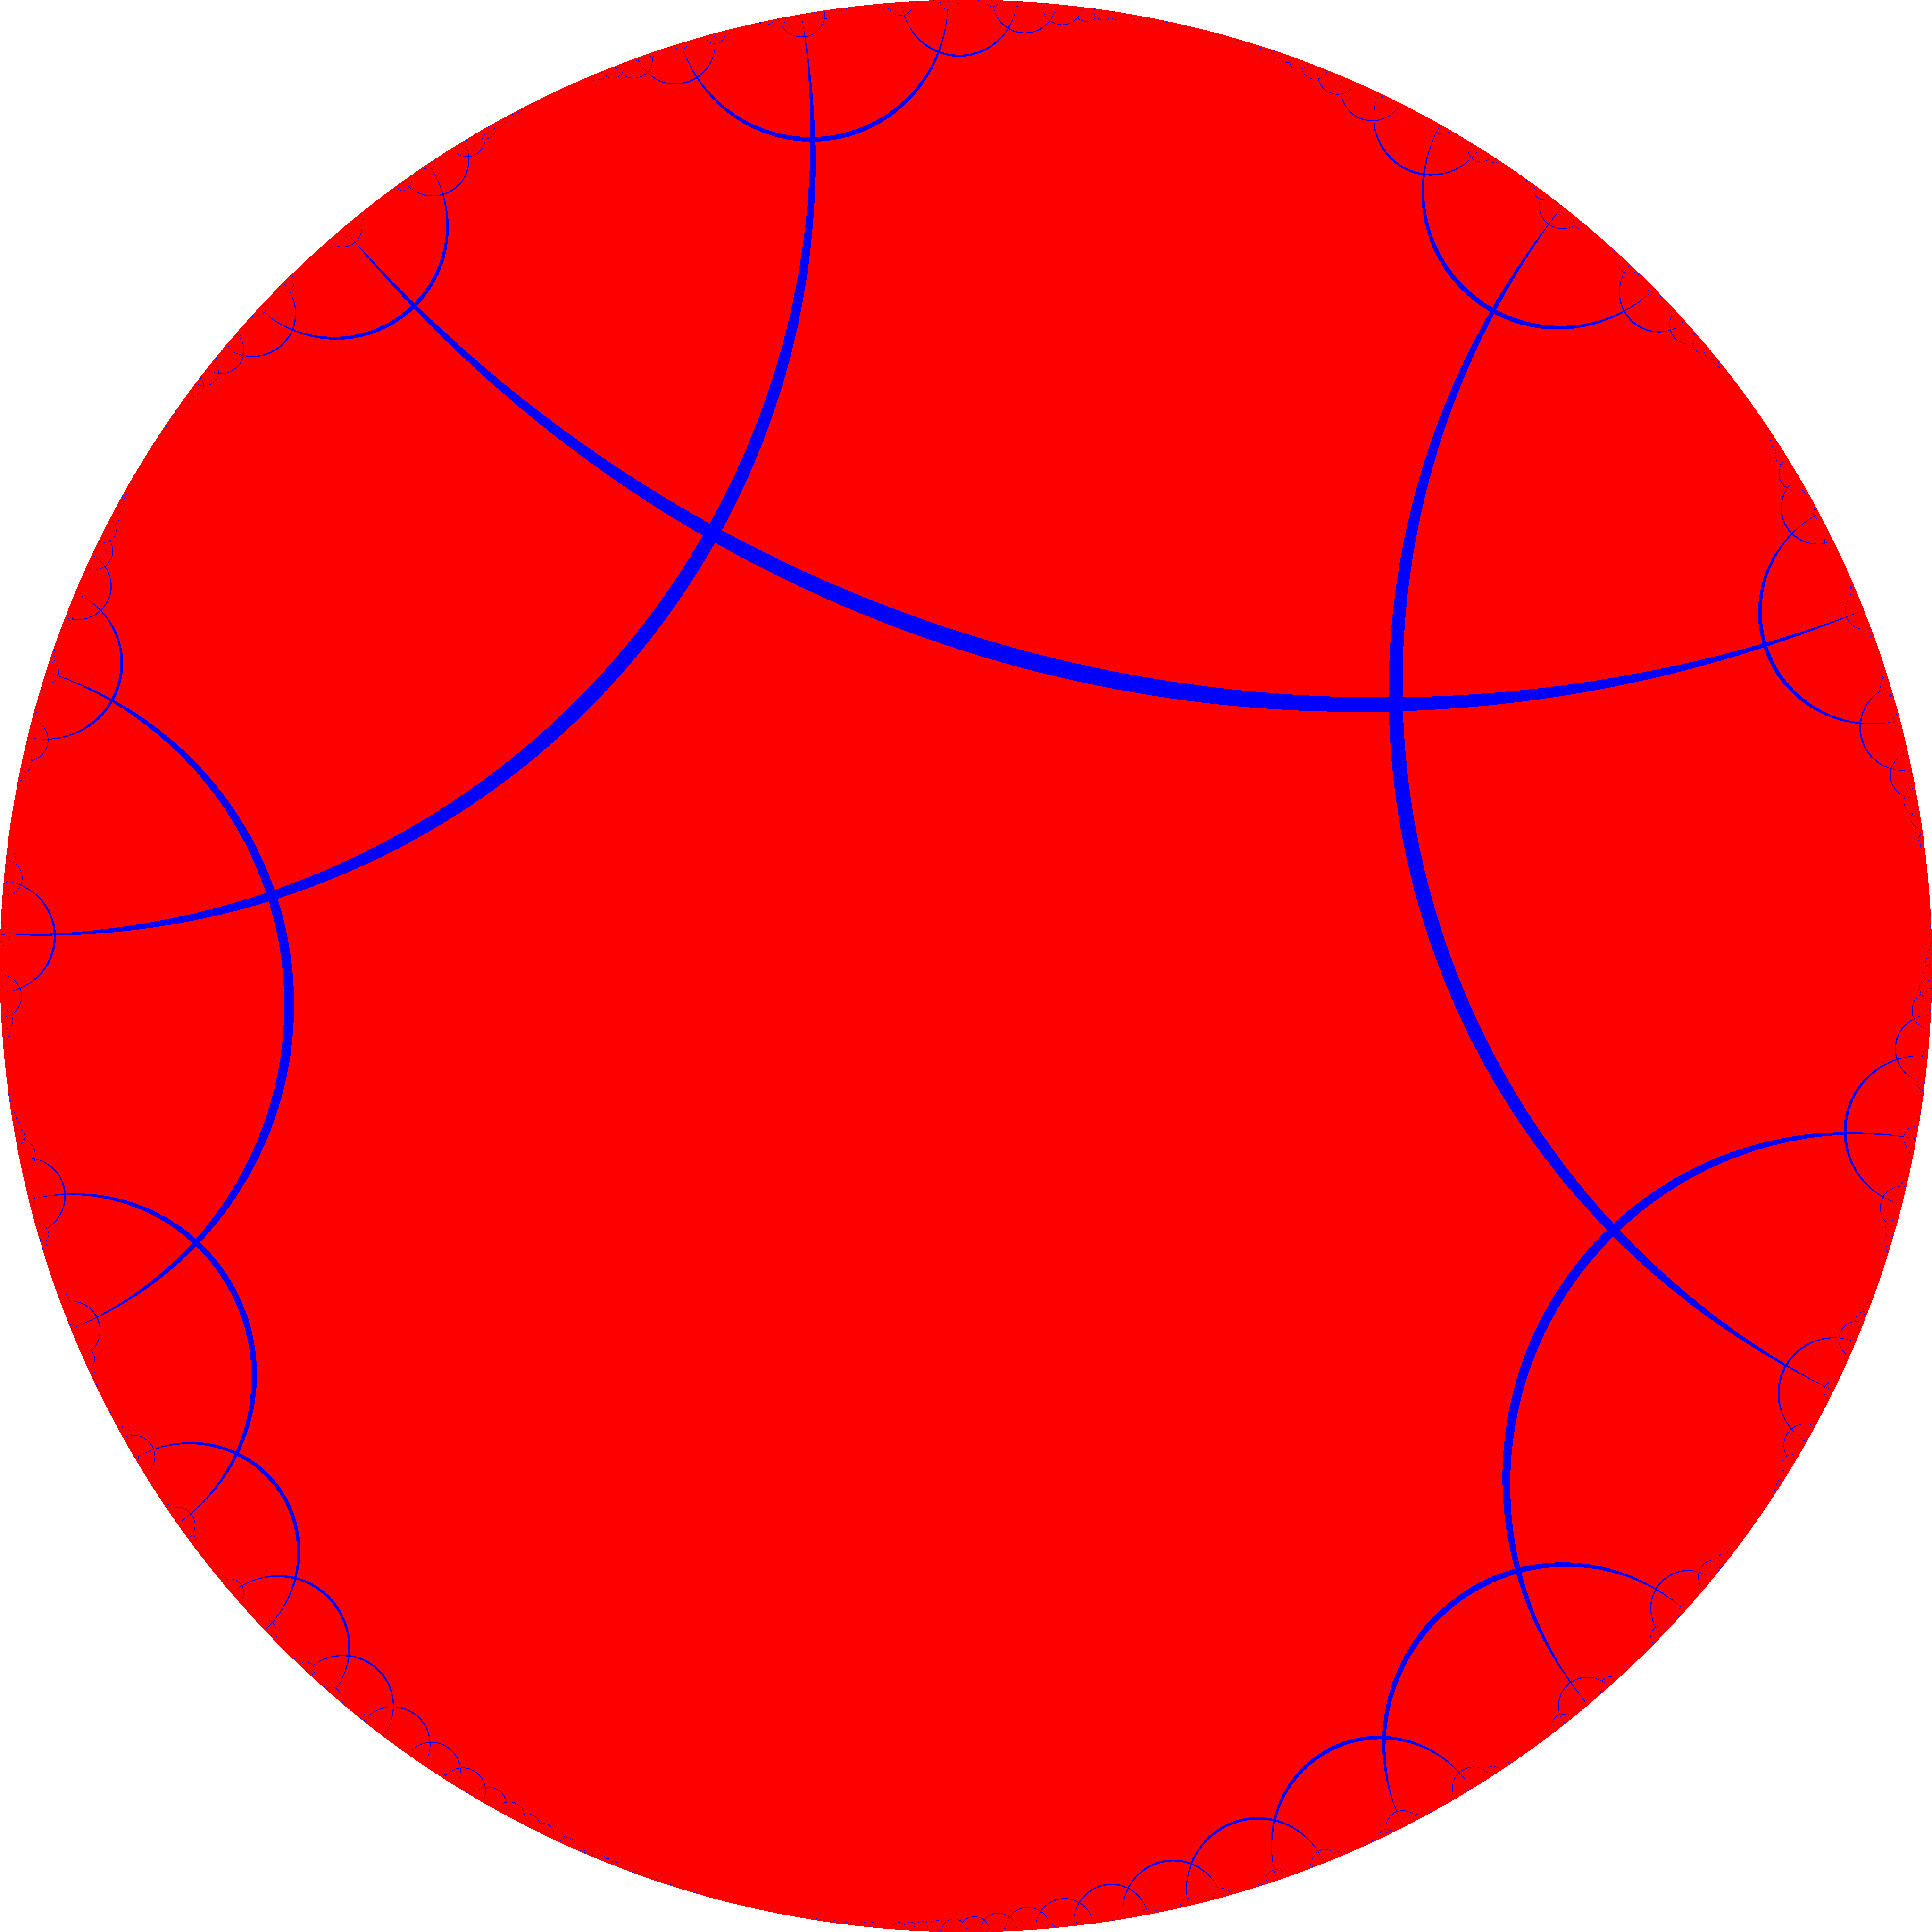
\includegraphics[width=6in]{images/t4096.png}};

    \draw [blue, dotted, thick]
          (-1.89, -7.39) node[circle, fill=blue, inner sep=1pt] (spole) {}
       -- (+0.00, +0.00) node[circle, fill=blue, inner sep=1pt] (orign) {}
       -- (+1.89, +7.39) node[circle, fill=blue, inner sep=1pt] (npole) {};

    %additional%
    \draw (-3.8, +6.0) node {3};
    \draw (-4.3, +4.7) node {4};
    \draw (-5.2, +4.7) node {5};

    %additional%
    \draw (-0.9, +6.2) node {1};
    \draw (-1.9, +2.9) node {2};
    \draw (-5.0, +0.3) node {3};
    \draw (-7.0, +0.0) node {4};

    %additional%
    \draw (+3.7, +4.9) node {0};
    \draw (+3.1, +1.7) node {1};
    \draw (+5.2, -2.5) node {2};

    %multiplicative%
    \draw (-6.2, +2.2) node {6};
    \draw (-5.35, -1.25) node {$\odot$ 2};
    \draw (-5.3, -2.2) node {3/2};

\end{tikzpicture}
\caption{嵌入整数}
\end{figure}

\newpage

\section{扩域的想法}

\subsection{基础元素}

$\begin{array}{|c|c|}\hline 1&\space\\\hline n&0\\\hline\end{array} \mapsto n$ 代表整数,整个树都是整数值 $n$

$\begin{array}{|c|c|}\hline0&\space\\\hline 1&0\\\hline\end{array} \mapsto h$ 代表全体横向测地线(加线)的过滤器

$\begin{array}{|c|c|}\hline0&\space\\\hline 0&1\\\hline\end{array} \mapsto i$ 代表全体横向测地线(加线)上的自然增加

$\begin{array}{|c|c|}\hline2&\space\\\hline 1&0\\\hline\end{array} \mapsto j$ 代表全体纵向测地线(乘线)上的自然增加

$\begin{array}{|c|c|}\hline2&\space\\\hline 0&1\\\hline\end{array} \mapsto q$

$p$ 是将 $q$ 的加乘位置互易得到

\subsubsection{问题}

$o_p$ 独点的过滤器存在吗?其中 $p$ 是从原点到达该点路径的二进制编码

$g_p$ 单独一条测地线的过滤器存在吗?其中 $p$ 是从原点到达测地线的路径的二进制编码

$n$ 自己可以构成域,$n$ 与 $q$ 的组合能生成域吗?$n$ 与 $p$、 $q$ 的组合能生成域吗?

生成域的目标是包含 surreal number。

\end{document}
